% Options for packages loaded elsewhere
\PassOptionsToPackage{unicode}{hyperref}
\PassOptionsToPackage{hyphens}{url}
\PassOptionsToPackage{dvipsnames,svgnames,x11names}{xcolor}
%
\documentclass[
  letterpaper,
  DIV=11,
  numbers=noendperiod,
  oneside]{scrartcl}

\usepackage{amsmath,amssymb}
\usepackage{iftex}
\ifPDFTeX
  \usepackage[T1]{fontenc}
  \usepackage[utf8]{inputenc}
  \usepackage{textcomp} % provide euro and other symbols
\else % if luatex or xetex
  \usepackage{unicode-math}
  \defaultfontfeatures{Scale=MatchLowercase}
  \defaultfontfeatures[\rmfamily]{Ligatures=TeX,Scale=1}
\fi
\usepackage{lmodern}
\ifPDFTeX\else  
    % xetex/luatex font selection
\fi
% Use upquote if available, for straight quotes in verbatim environments
\IfFileExists{upquote.sty}{\usepackage{upquote}}{}
\IfFileExists{microtype.sty}{% use microtype if available
  \usepackage[]{microtype}
  \UseMicrotypeSet[protrusion]{basicmath} % disable protrusion for tt fonts
}{}
\makeatletter
\@ifundefined{KOMAClassName}{% if non-KOMA class
  \IfFileExists{parskip.sty}{%
    \usepackage{parskip}
  }{% else
    \setlength{\parindent}{0pt}
    \setlength{\parskip}{6pt plus 2pt minus 1pt}}
}{% if KOMA class
  \KOMAoptions{parskip=half}}
\makeatother
\usepackage{xcolor}
\usepackage[left=1in,marginparwidth=2.0666666666667in,textwidth=4.1333333333333in,marginparsep=0.3in]{geometry}
\setlength{\emergencystretch}{3em} % prevent overfull lines
\setcounter{secnumdepth}{-\maxdimen} % remove section numbering
% Make \paragraph and \subparagraph free-standing
\ifx\paragraph\undefined\else
  \let\oldparagraph\paragraph
  \renewcommand{\paragraph}[1]{\oldparagraph{#1}\mbox{}}
\fi
\ifx\subparagraph\undefined\else
  \let\oldsubparagraph\subparagraph
  \renewcommand{\subparagraph}[1]{\oldsubparagraph{#1}\mbox{}}
\fi

\usepackage{color}
\usepackage{fancyvrb}
\newcommand{\VerbBar}{|}
\newcommand{\VERB}{\Verb[commandchars=\\\{\}]}
\DefineVerbatimEnvironment{Highlighting}{Verbatim}{commandchars=\\\{\}}
% Add ',fontsize=\small' for more characters per line
\usepackage{framed}
\definecolor{shadecolor}{RGB}{241,243,245}
\newenvironment{Shaded}{\begin{snugshade}}{\end{snugshade}}
\newcommand{\AlertTok}[1]{\textcolor[rgb]{0.68,0.00,0.00}{#1}}
\newcommand{\AnnotationTok}[1]{\textcolor[rgb]{0.37,0.37,0.37}{#1}}
\newcommand{\AttributeTok}[1]{\textcolor[rgb]{0.40,0.45,0.13}{#1}}
\newcommand{\BaseNTok}[1]{\textcolor[rgb]{0.68,0.00,0.00}{#1}}
\newcommand{\BuiltInTok}[1]{\textcolor[rgb]{0.00,0.23,0.31}{#1}}
\newcommand{\CharTok}[1]{\textcolor[rgb]{0.13,0.47,0.30}{#1}}
\newcommand{\CommentTok}[1]{\textcolor[rgb]{0.37,0.37,0.37}{#1}}
\newcommand{\CommentVarTok}[1]{\textcolor[rgb]{0.37,0.37,0.37}{\textit{#1}}}
\newcommand{\ConstantTok}[1]{\textcolor[rgb]{0.56,0.35,0.01}{#1}}
\newcommand{\ControlFlowTok}[1]{\textcolor[rgb]{0.00,0.23,0.31}{#1}}
\newcommand{\DataTypeTok}[1]{\textcolor[rgb]{0.68,0.00,0.00}{#1}}
\newcommand{\DecValTok}[1]{\textcolor[rgb]{0.68,0.00,0.00}{#1}}
\newcommand{\DocumentationTok}[1]{\textcolor[rgb]{0.37,0.37,0.37}{\textit{#1}}}
\newcommand{\ErrorTok}[1]{\textcolor[rgb]{0.68,0.00,0.00}{#1}}
\newcommand{\ExtensionTok}[1]{\textcolor[rgb]{0.00,0.23,0.31}{#1}}
\newcommand{\FloatTok}[1]{\textcolor[rgb]{0.68,0.00,0.00}{#1}}
\newcommand{\FunctionTok}[1]{\textcolor[rgb]{0.28,0.35,0.67}{#1}}
\newcommand{\ImportTok}[1]{\textcolor[rgb]{0.00,0.46,0.62}{#1}}
\newcommand{\InformationTok}[1]{\textcolor[rgb]{0.37,0.37,0.37}{#1}}
\newcommand{\KeywordTok}[1]{\textcolor[rgb]{0.00,0.23,0.31}{#1}}
\newcommand{\NormalTok}[1]{\textcolor[rgb]{0.00,0.23,0.31}{#1}}
\newcommand{\OperatorTok}[1]{\textcolor[rgb]{0.37,0.37,0.37}{#1}}
\newcommand{\OtherTok}[1]{\textcolor[rgb]{0.00,0.23,0.31}{#1}}
\newcommand{\PreprocessorTok}[1]{\textcolor[rgb]{0.68,0.00,0.00}{#1}}
\newcommand{\RegionMarkerTok}[1]{\textcolor[rgb]{0.00,0.23,0.31}{#1}}
\newcommand{\SpecialCharTok}[1]{\textcolor[rgb]{0.37,0.37,0.37}{#1}}
\newcommand{\SpecialStringTok}[1]{\textcolor[rgb]{0.13,0.47,0.30}{#1}}
\newcommand{\StringTok}[1]{\textcolor[rgb]{0.13,0.47,0.30}{#1}}
\newcommand{\VariableTok}[1]{\textcolor[rgb]{0.07,0.07,0.07}{#1}}
\newcommand{\VerbatimStringTok}[1]{\textcolor[rgb]{0.13,0.47,0.30}{#1}}
\newcommand{\WarningTok}[1]{\textcolor[rgb]{0.37,0.37,0.37}{\textit{#1}}}

\providecommand{\tightlist}{%
  \setlength{\itemsep}{0pt}\setlength{\parskip}{0pt}}\usepackage{longtable,booktabs,array}
\usepackage{calc} % for calculating minipage widths
% Correct order of tables after \paragraph or \subparagraph
\usepackage{etoolbox}
\makeatletter
\patchcmd\longtable{\par}{\if@noskipsec\mbox{}\fi\par}{}{}
\makeatother
% Allow footnotes in longtable head/foot
\IfFileExists{footnotehyper.sty}{\usepackage{footnotehyper}}{\usepackage{footnote}}
\makesavenoteenv{longtable}
\usepackage{graphicx}
\makeatletter
\def\maxwidth{\ifdim\Gin@nat@width>\linewidth\linewidth\else\Gin@nat@width\fi}
\def\maxheight{\ifdim\Gin@nat@height>\textheight\textheight\else\Gin@nat@height\fi}
\makeatother
% Scale images if necessary, so that they will not overflow the page
% margins by default, and it is still possible to overwrite the defaults
% using explicit options in \includegraphics[width, height, ...]{}
\setkeys{Gin}{width=\maxwidth,height=\maxheight,keepaspectratio}
% Set default figure placement to htbp
\makeatletter
\def\fps@figure{htbp}
\makeatother
\newlength{\cslhangindent}
\setlength{\cslhangindent}{1.5em}
\newlength{\csllabelwidth}
\setlength{\csllabelwidth}{3em}
\newlength{\cslentryspacingunit} % times entry-spacing
\setlength{\cslentryspacingunit}{\parskip}
\newenvironment{CSLReferences}[2] % #1 hanging-ident, #2 entry spacing
 {% don't indent paragraphs
  \setlength{\parindent}{0pt}
  % turn on hanging indent if param 1 is 1
  \ifodd #1
  \let\oldpar\par
  \def\par{\hangindent=\cslhangindent\oldpar}
  \fi
  % set entry spacing
  \setlength{\parskip}{#2\cslentryspacingunit}
 }%
 {}
\usepackage{calc}
\newcommand{\CSLBlock}[1]{#1\hfill\break}
\newcommand{\CSLLeftMargin}[1]{\parbox[t]{\csllabelwidth}{#1}}
\newcommand{\CSLRightInline}[1]{\parbox[t]{\linewidth - \csllabelwidth}{#1}\break}
\newcommand{\CSLIndent}[1]{\hspace{\cslhangindent}#1}

\usepackage{booktabs}
\usepackage{longtable}
\usepackage{array}
\usepackage{multirow}
\usepackage{wrapfig}
\usepackage{float}
\usepackage{colortbl}
\usepackage{pdflscape}
\usepackage{tabu}
\usepackage{threeparttable}
\usepackage{threeparttablex}
\usepackage[normalem]{ulem}
\usepackage{makecell}
\usepackage{xcolor}
\KOMAoption{captions}{tableheading}
\makeatletter
\makeatother
\makeatletter
\makeatother
\makeatletter
\@ifpackageloaded{caption}{}{\usepackage{caption}}
\AtBeginDocument{%
\ifdefined\contentsname
  \renewcommand*\contentsname{Table of contents}
\else
  \newcommand\contentsname{Table of contents}
\fi
\ifdefined\listfigurename
  \renewcommand*\listfigurename{List of Figures}
\else
  \newcommand\listfigurename{List of Figures}
\fi
\ifdefined\listtablename
  \renewcommand*\listtablename{List of Tables}
\else
  \newcommand\listtablename{List of Tables}
\fi
\ifdefined\figurename
  \renewcommand*\figurename{Figure}
\else
  \newcommand\figurename{Figure}
\fi
\ifdefined\tablename
  \renewcommand*\tablename{Table}
\else
  \newcommand\tablename{Table}
\fi
}
\@ifpackageloaded{float}{}{\usepackage{float}}
\floatstyle{ruled}
\@ifundefined{c@chapter}{\newfloat{codelisting}{h}{lop}}{\newfloat{codelisting}{h}{lop}[chapter]}
\floatname{codelisting}{Listing}
\newcommand*\listoflistings{\listof{codelisting}{List of Listings}}
\makeatother
\makeatletter
\@ifpackageloaded{caption}{}{\usepackage{caption}}
\@ifpackageloaded{subcaption}{}{\usepackage{subcaption}}
\makeatother
\makeatletter
\@ifpackageloaded{tcolorbox}{}{\usepackage[skins,breakable]{tcolorbox}}
\makeatother
\makeatletter
\@ifundefined{shadecolor}{\definecolor{shadecolor}{rgb}{.97, .97, .97}}
\makeatother
\makeatletter
\makeatother
\makeatletter
\@ifpackageloaded{sidenotes}{}{\usepackage{sidenotes}}
\@ifpackageloaded{marginnote}{}{\usepackage{marginnote}}
\makeatother
\makeatletter
\makeatother
\ifLuaTeX
  \usepackage{selnolig}  % disable illegal ligatures
\fi
\IfFileExists{bookmark.sty}{\usepackage{bookmark}}{\usepackage{hyperref}}
\IfFileExists{xurl.sty}{\usepackage{xurl}}{} % add URL line breaks if available
\urlstyle{same} % disable monospaced font for URLs
\hypersetup{
  pdftitle={Report on the use of passive acoustic monitoring in Prince Edward Island National Park},
  pdfauthor={Alex MacPhail},
  colorlinks=true,
  linkcolor={blue},
  filecolor={Maroon},
  citecolor={Blue},
  urlcolor={Blue},
  pdfcreator={LaTeX via pandoc}}

\title{Report on the use of passive acoustic monitoring in Prince Edward
Island National Park}
\author{Alex MacPhail}
\date{2024-02-06}

\begin{document}
\maketitle
\ifdefined\Shaded\renewenvironment{Shaded}{\begin{tcolorbox}[borderline west={3pt}{0pt}{shadecolor}, breakable, frame hidden, sharp corners, enhanced, boxrule=0pt, interior hidden]}{\end{tcolorbox}}\fi

\renewcommand*\contentsname{Table of contents}
{
\hypersetup{linkcolor=}
\setcounter{tocdepth}{3}
\tableofcontents
}
\begin{figure}

{\centering 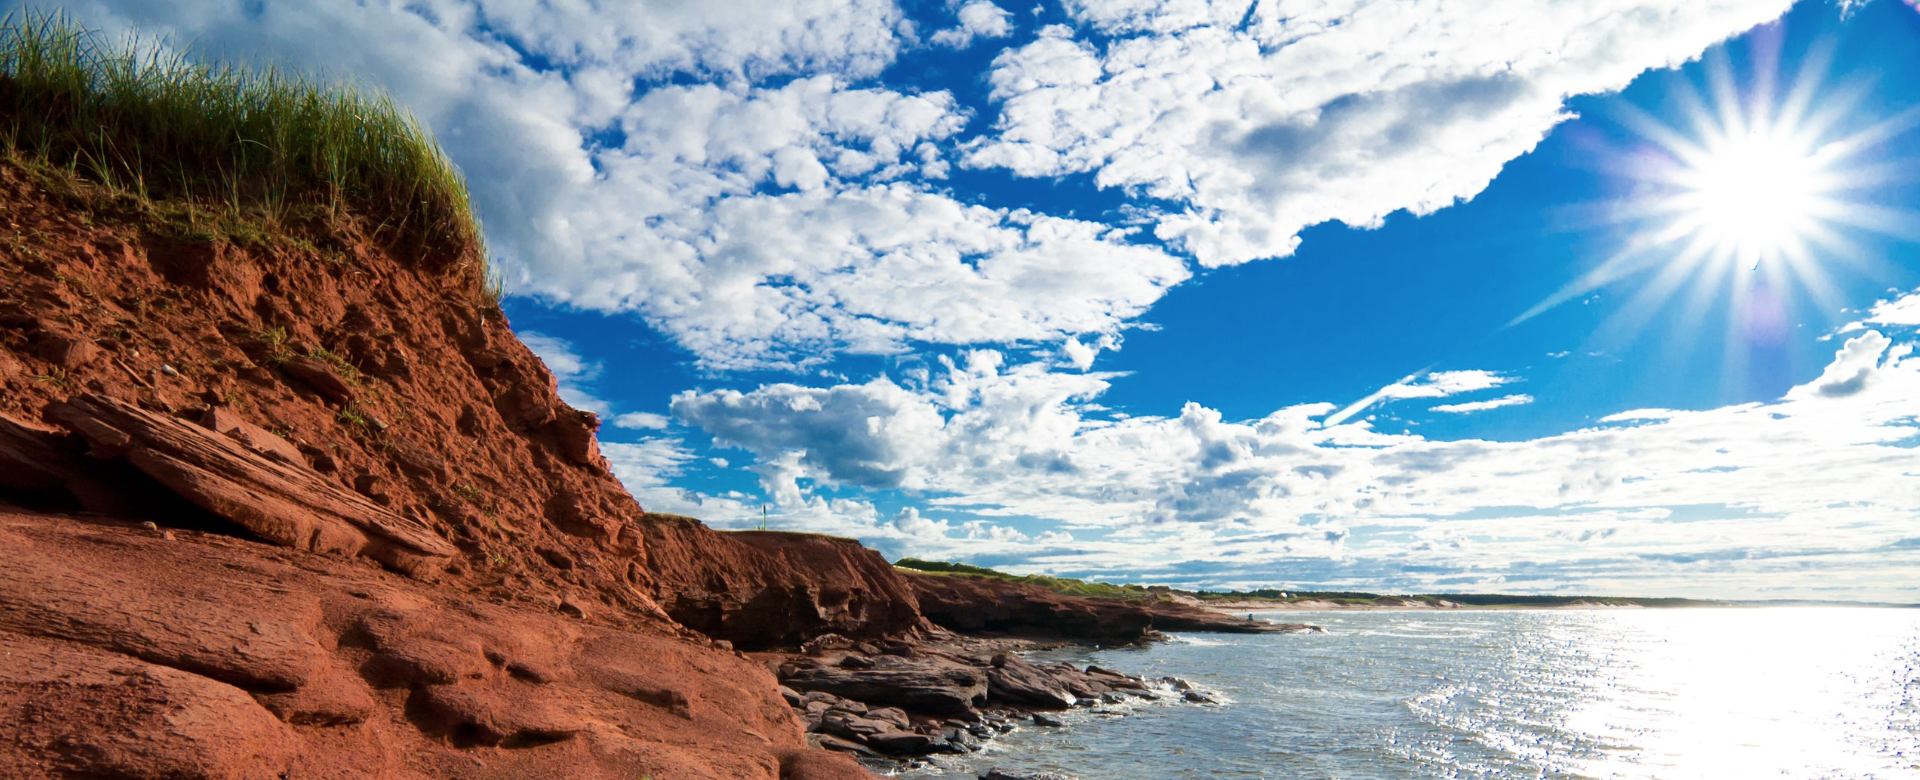
\includegraphics{peinpheader.png}

}

\end{figure}

To run this report locally:

\begin{itemize}
\tightlist
\item
  Open RStudio or your preferred IDE
\item
  Create a new project and set up for version control using the GitHub
  repository
\item
  Pull from remote main
\item
  Load the \texttt{pei.RData} file in the first chunk
\item
  Render the document and review the results
\end{itemize}

\hypertarget{abstract}{%
\section{Abstract}\label{abstract}}

Passive acoustic monitoring has proven to be a valuable tool for
monitoring vocalizing species. Environmental sensors are becoming
increasingly easy to program and can autonomously generating extensive
data sets of the soundscape, an invaluable resource for ecological
integrity monitoring. Prince Edward Island National deployed autonomous
recording units (ARUs) across 30 locations during a comprehensive
five-year survey. The analysis revealed that species richness and
diversity remained relatively stable, while single-species species
occupancy exhibited diverse patterns. Common and generalist species
showed consistent occupancy, but there was a notable reduction in
conifer-nesting species in 2023, likely attributed to forest structural
loss. Ongoing monitoring and dynamic models can yield more detailed and
predictive results to ensure the continued maintenance of ecological
integrity in the Park.

\begin{center}\rule{0.5\linewidth}{0.5pt}\end{center}

\hypertarget{land-acknowledgement}{%
\section{Land Acknowledgement}\label{land-acknowledgement}}

In the spirit of Reconciliation, we\,acknowledge that the\,land\,upon
which this data was gathered is unceeded Mi'kmaq territory. Epekwitk
(Prince Edward Island), Mi'kma'ki, is covered by the historic Treaties
of Peace and Friendship. We pay our respects to the Indigenous Mi'kmaq
People who have occupied this Island\,for over 12,000 years; past,
present and future.

\hypertarget{introduction}{%
\section{Introduction}\label{introduction}}

Human activities have been identified as key pressures and contributors
to the global decline in forest wildlife (Allan et al.
(2017)\marginpar{\begin{footnotesize}\leavevmode\vadjust pre{\protect\hypertarget{ref-allan2017recent}{}}%
Allan, James R, Oscar Venter, Sean Maxwell, Bastian Bertzky, Kendall
Jones, Yichuan Shi, and James EM Watson. 2017. {``Recent Increases in
Human Pressure and Forest Loss Threaten Many Natural World Heritage
Sites.''} \emph{Biological Conservation} 206: 47--55.\vspace{2mm}\par\end{footnotesize}}).
The repercussions of habitat fragmentation (Fahrig
(2003)\marginpar{\begin{footnotesize}\leavevmode\vadjust pre{\protect\hypertarget{ref-fahrig2003effects}{}}%
Fahrig, Lenore. 2003. {``Effects of Habitat Fragmentation on
Biodiversity.''} \emph{Annual Review of Ecology, Evolution, and
Systematics} 34 (1): 487--515.\vspace{2mm}\par\end{footnotesize}})
and loss (Hanski
(2011)\marginpar{\begin{footnotesize}\leavevmode\vadjust pre{\protect\hypertarget{ref-hanski2011habitat}{}}%
Hanski, Ilkka. 2011. {``Habitat Loss, the Dynamics of Biodiversity, and
a Perspective on Conservation.''} \emph{Ambio} 40 (3): 248--55.\vspace{2mm}\par\end{footnotesize}}),
climate change (Mantyka-pringle, Martin, and Rhodes
(2012)\marginpar{\begin{footnotesize}\leavevmode\vadjust pre{\protect\hypertarget{ref-mantyka2012interactions}{}}%
Mantyka-pringle, Chrystal S, Tara G Martin, and Jonathan R Rhodes. 2012.
{``Interactions Between Climate and Habitat Loss Effects on
Biodiversity: A Systematic Review and Meta-Analysis.''} \emph{Global
Change Biology} 18 (4): 1239--52.\vspace{2mm}\par\end{footnotesize}},
Sattar et al.
(2021)\marginpar{\begin{footnotesize}\leavevmode\vadjust pre{\protect\hypertarget{ref-sattar2021review}{}}%
Sattar, Q, ME Maqbool, R Ehsan, S Akhtar, Q Sattar, ME Maqbool, R Ehsan,
and S Akhtar. 2021. {``Review on Climate Change and Its Effect on
Wildlife and Ecosystem.''} \emph{Open J Environ Biol} 6 (1): 008--14.\vspace{2mm}\par\end{footnotesize}},
Abrahms et al.
(2023)\marginpar{\begin{footnotesize}\leavevmode\vadjust pre{\protect\hypertarget{ref-abrahms2023climate}{}}%
Abrahms, Briana, Neil H Carter, TJ Clark-Wolf, Kaitlyn M Gaynor, Erik
Johansson, Alex McInturff, Anna C Nisi, Kasim Rafiq, and Leigh West.
2023. {``Climate Change as a Global Amplifier of Human--Wildlife
Conflict.''} \emph{Nature Climate Change} 13 (3): 224--34.\vspace{2mm}\par\end{footnotesize}}),
and increased access to sensitive areas exert direct and indirect
pressures on forest biodiversity, particularly in managed regions in
Canada (Lemieux et al.
(2011)\marginpar{\begin{footnotesize}\leavevmode\vadjust pre{\protect\hypertarget{ref-lemieux2011state}{}}%
Lemieux, Christopher J, Thomas J Beechey, Daniel J Scott, and Paul A
Gray. 2011. {``The State of Climate Change Adaptation in Canada's
Protected Areas Sector.''} \emph{The Canadian Geographer/Le G{é}ographe
Canadien} 55 (3): 301--17.\vspace{2mm}\par\end{footnotesize}}).

In 2019, Prince Edward Island National Park initiated a program
incorporating autonomous recording units (ARUs) for passive acoustic
monitoring (PAM) of the Park's wildlife. ARUs are compact environmental
sensors that are designed to passively record the environment (Shonfield
and Bayne
(2017)\marginpar{\begin{footnotesize}\leavevmode\vadjust pre{\protect\hypertarget{ref-aru-overview}{}}%
Shonfield, Julia, and Erin M Bayne. 2017. {``Autonomous Recording Units
in Avian Ecological Research: Current Use and Future Applications.''}
\emph{Avian Conservation \& Ecology} 12 (1).\vspace{2mm}\par\end{footnotesize}}),
capturing vocalizing species like birds and amphibians, which is growing
in use across the globe (Sugai et al.
(2018)\marginpar{\begin{footnotesize}\leavevmode\vadjust pre{\protect\hypertarget{ref-lots-of-pam}{}}%
Sugai, Larissa Sayuri Moreira, Thiago Sanna Freire Silva, Jr Ribeiro
José Wagner, and Diego Llusia. 2018. {``{Terrestrial Passive Acoustic
Monitoring: Review and Perspectives}.''} \emph{BioScience} 69 (1):
15--25. \url{https://doi.org/10.1093/biosci/biy147}.\vspace{2mm}\par\end{footnotesize}}).
This technology enables resource managers to conduct prolonged surveys
with minimal human interference. The subsequent data collected by these
units contribute valuable information to ecological integrity metrics
such as species richness, diversity, occupancy, and trends over time.
This data aids decision-making and management within the Park. Given the
rapid and ease of accumulating data from these units, maintaining a high
standard of data integrity is paramount to ensure future data
interoperability and sharing. \href{https://www.wildtrax.ca}{WildTrax}
is an online platform developed by the \href{https://abmi.ca}{Alberta
Biodiversity Monitoring Institute (\textbf{ABMI})} for users of
environmental sensors to help addresses these big data challenges by
providing solutions to standardize, harmonize, and share data.

The objectives of this report are to:

\begin{itemize}
\tightlist
\item
  Describe the data management and processing procedures for the
  acoustic data collected from 2019 to 2023;
\item
  Utilize traditional human tagging, visual scanning and automated
  recognition techniques to detect and count species and individuals
  heard on recordings;
\item
  Define straightforward methods for evaluating species presence,
  species richness, and species occupancy over time at various
  locations;
\item
  Offer recommendations for ongoing monitoring approaches to contribute
  to the assessment of ecological integrity in forest ecosystems;
\item
  Facilitate data publication to the public, resource managers, academic
  institutions, and any other relevant agencies
\end{itemize}

\begin{center}\rule{0.5\linewidth}{0.5pt}\end{center}

\hypertarget{methods}{%
\section{Methods}\label{methods}}

\hypertarget{data-collection}{%
\subsection{Data collection}\label{data-collection}}

Data were collected during the spring and summer seasons from 2019 to
2023. A total of 30 locations were surveyed over the five-year period:

\begin{itemize}
\tightlist
\item
  21 locations as part of the forest songbird monitoring program (code:
  \texttt{PENP-*}) with ARUs recording during the morning hours,
\item
  6 for Bank Swallow Monitoring (code: \texttt{PENP-BS-*}) with ARUs
  placed strategically beside ponds recording in the evening,
\item
  2 locations deployed in First Nations communities
  (\texttt{ASC-1,\ LXI-1}) to complement the forest songbird and evening
  schedules,
\item
  And one location (\texttt{PENP-E1}), which was to examine the effects
  of a single public event
\end{itemize}

Locations were surveyed on rotation with 9 locations (PENP-1-1,
PENP-1-2, PENP-2-3, PENP-3-1, PENP-3-2, PENP-4-1, PENP-4-2, PENP-4-3,
PENP-4-4) surveyed each year. A detailed list of all survey years can be
found in Table 1 (Table~\ref{tbl-loc-summary}) and illustrated in Figure
1 (Figure~\ref{fig-locs}). ARUs were deployed at the beginning of the
breeding season in April-May, and rotated locations until their final
retrieval in July-August. At the forest songbird locations
(\texttt{PENP-*}), the ARUs were set to record for 30 minutes
continuously every hour for four hours, starting one hour before dawn
and ending three hours after dawn. For Bank Swallow Monitoring locations
(\texttt{PENP-BS}), recordings were made every 5 minutes for a duration
of 3 minutes each from 1.5 hours before dusk to 1.5 hours after dusk. On
average, each ARU recorded for 11.27 +/- 8.03 days.

\begin{figure}

\sidecaption{\label{fig-locs}ARU monitoring locations surveyed each year
as part of the songbird monitoring program.}

{\centering 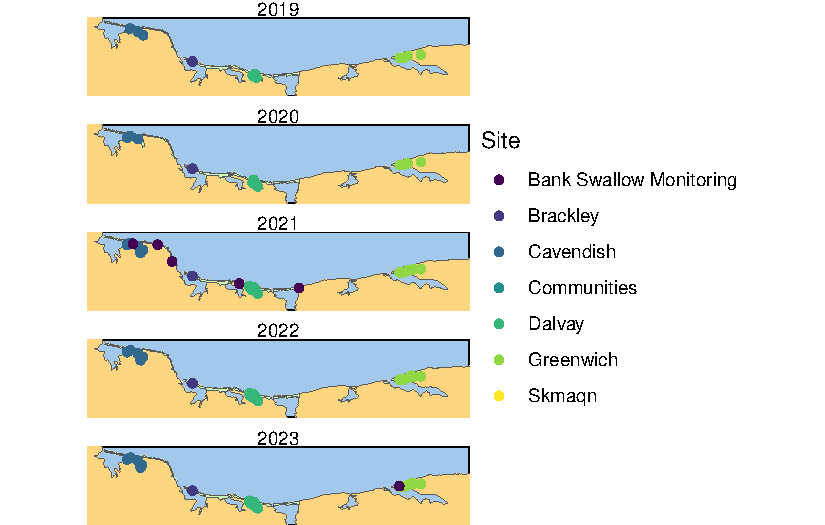
\includegraphics{peinp_files/figure-pdf/fig-locs-1.pdf}

}

\end{figure}

\hypertarget{tbl-loc-summary}{}
\begin{table}

\caption{\label{tbl-loc-summary}Locations surveyed across years. Ones indicated a deployment in that
year for that location }Location summary for ARUs deployed}
\centering
\begin{tabular}[t]{l|r|r|r|r|r|l}
\hline
Location & 2019 & 2020 & 2021 & 2022 & 2023 & Site\\
\hline
PENP-1-1 & 1 & 1 & 1 & 1 & 1 & Cavendish\\
\hline
PENP-1-2 & 1 & 1 & 1 & 1 & 1 & Cavendish\\
\hline
PENP-1-3 & 1 & 0 & 1 & 1 & 0 & Cavendish\\
\hline
PENP-2-3 & 1 & 1 & 1 & 1 & 1 & Brackley\\
\hline
PENP-3-1 & 1 & 1 & 1 & 1 & 1 & Dalvay\\
\hline
PENP-3-2 & 1 & 1 & 1 & 1 & 1 & Dalvay\\
\hline
PENP-3-4 & 1 & 0 & 1 & 1 & 1 & Dalvay\\
\hline
PENP-4-1 & 1 & 1 & 1 & 1 & 1 & Greenwich\\
\hline
PENP-4-2 & 1 & 1 & 1 & 1 & 1 & Greenwich\\
\hline
PENP-4-3 & 1 & 1 & 1 & 1 & 1 & Greenwich\\
\hline
PENP-4-4 & 1 & 1 & 1 & 1 & 1 & Greenwich\\
\hline
PENP-1-4 & 0 & 1 & 1 & 1 & 1 & Cavendish\\
\hline
PENP-3-5 & 0 & 1 & 1 & 1 & 1 & Dalvay\\
\hline
PENP-3-6 & 0 & 1 & 1 & 1 & 1 & Dalvay\\
\hline
ASC-1 & 0 & 0 & 1 & 0 & 0 & Communities\\
\hline
LXI-1 & 0 & 0 & 1 & 0 & 0 & Communities\\
\hline
PENP-1-5 & 0 & 0 & 1 & 1 & 1 & Cavendish\\
\hline
PENP-1-6 & 0 & 0 & 1 & 1 & 1 & Cavendish\\
\hline
PENP-3-7 & 0 & 0 & 1 & 1 & 1 & Dalvay\\
\hline
PENP-3-8 & 0 & 0 & 1 & 1 & 1 & Dalvay\\
\hline
PENP-4-6 & 0 & 0 & 1 & 1 & 1 & Greenwich\\
\hline
PENP-5-1 & 0 & 0 & 1 & 1 & 1 & Skmaqn\\
\hline
PENP-BS-1 & 0 & 0 & 1 & 0 & 0 & Bank Swallow Monitoring\\
\hline
PENP-BS-2 & 0 & 0 & 1 & 0 & 0 & Bank Swallow Monitoring\\
\hline
PENP-BS-3 & 0 & 0 & 1 & 0 & 0 & Bank Swallow Monitoring\\
\hline
PENP-BS-4 & 0 & 0 & 1 & 0 & 0 & Bank Swallow Monitoring\\
\hline
PENP-BS-5 & 0 & 0 & 1 & 0 & 0 & Bank Swallow Monitoring\\
\hline
PENP-4-5 & 0 & 0 & 0 & 1 & 1 & Greenwich\\
\hline
PENP-E1 & 0 & 0 & 0 & 1 & 0 & Skmaqn\\
\hline
PENP-BS-6 & 0 & 0 & 0 & 0 & 1 & Bank Swallow Monitoring\\
\hline
\end{tabular}
\end{table}

\hypertarget{tbl-obvs-and-covs}{}
\begin{table}

\caption{\label{tbl-obvs-and-covs}Site covariates for each forest songbird monitoring (PENP-*) location.
Landcover is measured as proportion cover at 150 meter radius
surrounding the ARU categorized into anthropogenic (pavement, soy), open
(grass, sand dune, bare soil), deciduous (red maple, white birch, alder,
poplar) and conifer (white spruce, black spruce, balsam fir). }Location summary for ARUs deployed}
\centering
\begin{tabular}[t]{l|r|r|r|r|r}
\hline
location & Distance from coast (m) & Anthro & Deciduous & Open & Conifer\\
\hline
PENP-1-1 & 751 & 0.05 & 0.60 & 0.35 & 0.00\\
\hline
PENP-1-2 & 491 & 0.06 & 0.00 & 0.00 & 0.94\\
\hline
PENP-1-3 & 1540 & 0.03 & 0.00 & 0.13 & 0.85\\
\hline
PENP-1-4 & 820 & 0.09 & 0.00 & 0.00 & 0.91\\
\hline
PENP-1-5 & 2050 & 0.00 & 0.91 & 0.01 & 0.08\\
\hline
PENP-1-6 & 1640 & 0.00 & 0.00 & 0.97 & 0.03\\
\hline
PENP-2-3 & 78 & 0.11 & 0.02 & 0.12 & 0.75\\
\hline
PENP-3-1 & 678 & 0.32 & 0.01 & 0.00 & 0.67\\
\hline
PENP-3-2 & 672 & 0.09 & 0.38 & 0.00 & 0.53\\
\hline
PENP-3-4 & 355 & 0.31 & 0.00 & 0.00 & 0.69\\
\hline
PENP-3-5 & 63 & 0.10 & 0.04 & 0.57 & 0.29\\
\hline
PENP-3-6 & 1198 & 0.00 & 0.46 & 0.00 & 0.54\\
\hline
PENP-3-7 & 408 & 0.02 & 0.00 & 0.10 & 0.89\\
\hline
PENP-3-8 & 65 & 0.39 & 0.00 & 0.17 & 0.43\\
\hline
PENP-4-1 & 447 & 0.00 & 0.34 & 0.25 & 0.41\\
\hline
PENP-4-2 & 912 & 0.00 & 0.05 & 0.21 & 0.75\\
\hline
PENP-4-3 & 1271 & 0.06 & 0.14 & 0.00 & 0.80\\
\hline
PENP-4-4 & 902 & 0.00 & 0.01 & 0.00 & 0.99\\
\hline
PENP-4-5 & 576 & 0.57 & 0.43 & 0.00 & 0.00\\
\hline
PENP-4-6 & 789 & 0.00 & 0.84 & 0.00 & 0.16\\
\hline
PENP-5-1 & 137 & 0.00 & 0.00 & 0.36 & 0.64\\
\hline
\end{tabular}
\end{table}

\hypertarget{data-management}{%
\subsection{Data management}\label{data-management}}

A total of 10078 recordings were collected (see
Figure~\ref{fig-recs-collect}). From 2019 - 2021, data were transferred
via hard drive to the University of Alberta in Edmonton, where they are
redundantly stored on a server known as Cirrus. The recordings were
standardized to ensure adherence to the naming convention of
\texttt{LOCATION\_DATETIME}, such as
\texttt{PENP-1-1\_20230625\_053500.wav}. The remaining recordings (2022
- 2023) were directly uploaded to WildTrax by Parks Canada staff and can
be downloaded from the platform's Recording tab, accessible under Manage
\textgreater{} Download list of recordings (see
Figure~\ref{fig-download-recs}).

\begin{figure}

{\centering 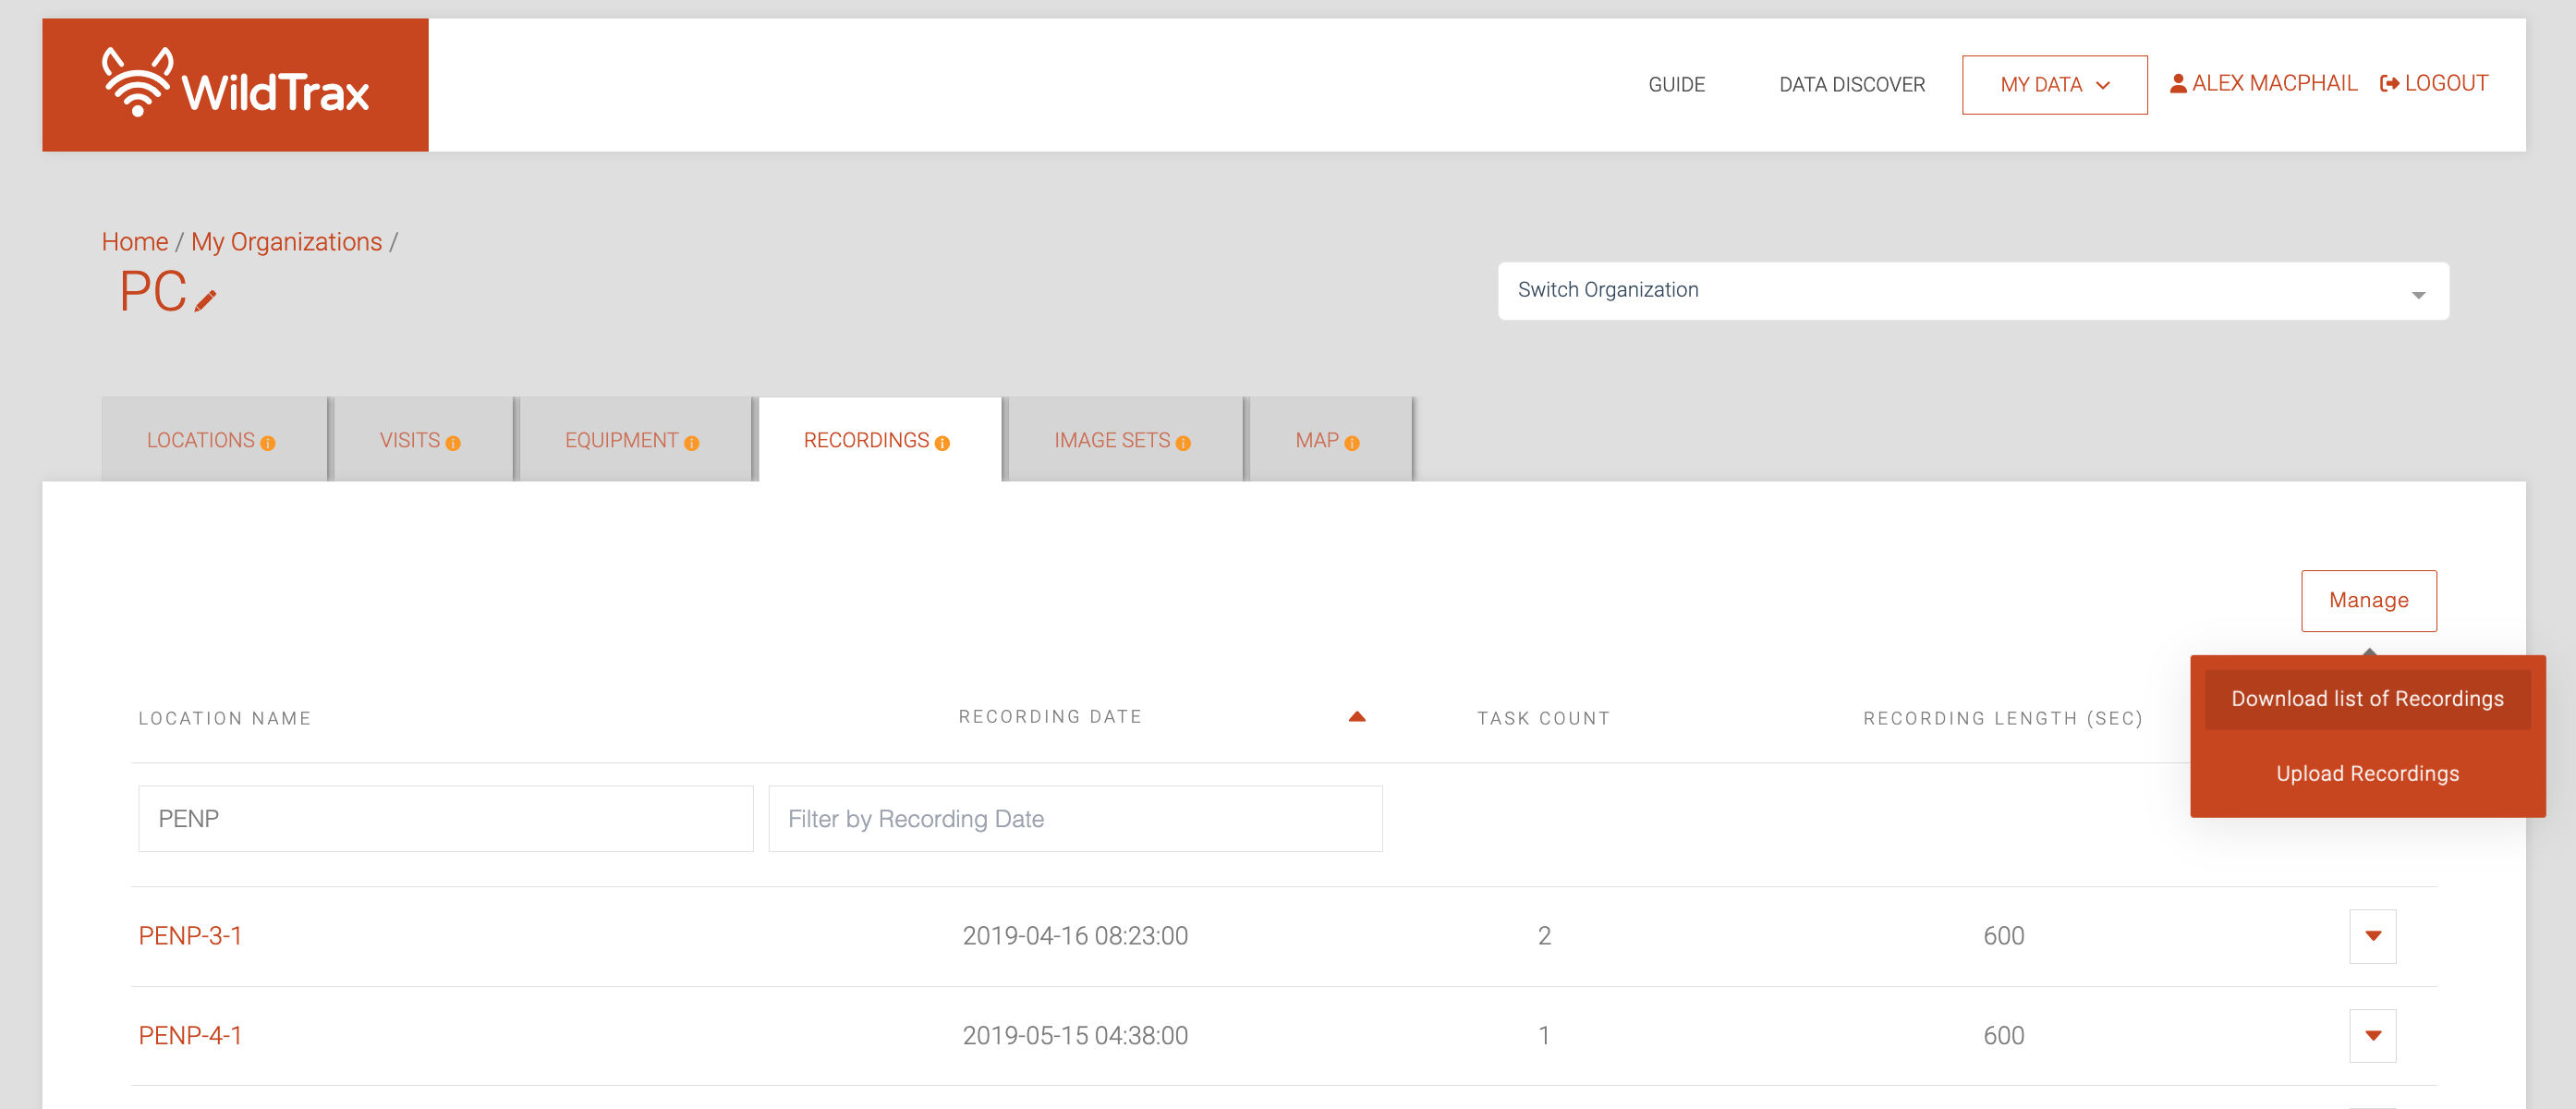
\includegraphics{download-recs.png}

}

\caption{\label{fig-download-recs}Downloading a list of recordings from
WildTrax}

\end{figure}

\begin{figure}

\sidecaption{\label{fig-recs-collect}Ridgeplot of recordings collected
for each location over each survey year}

{\centering 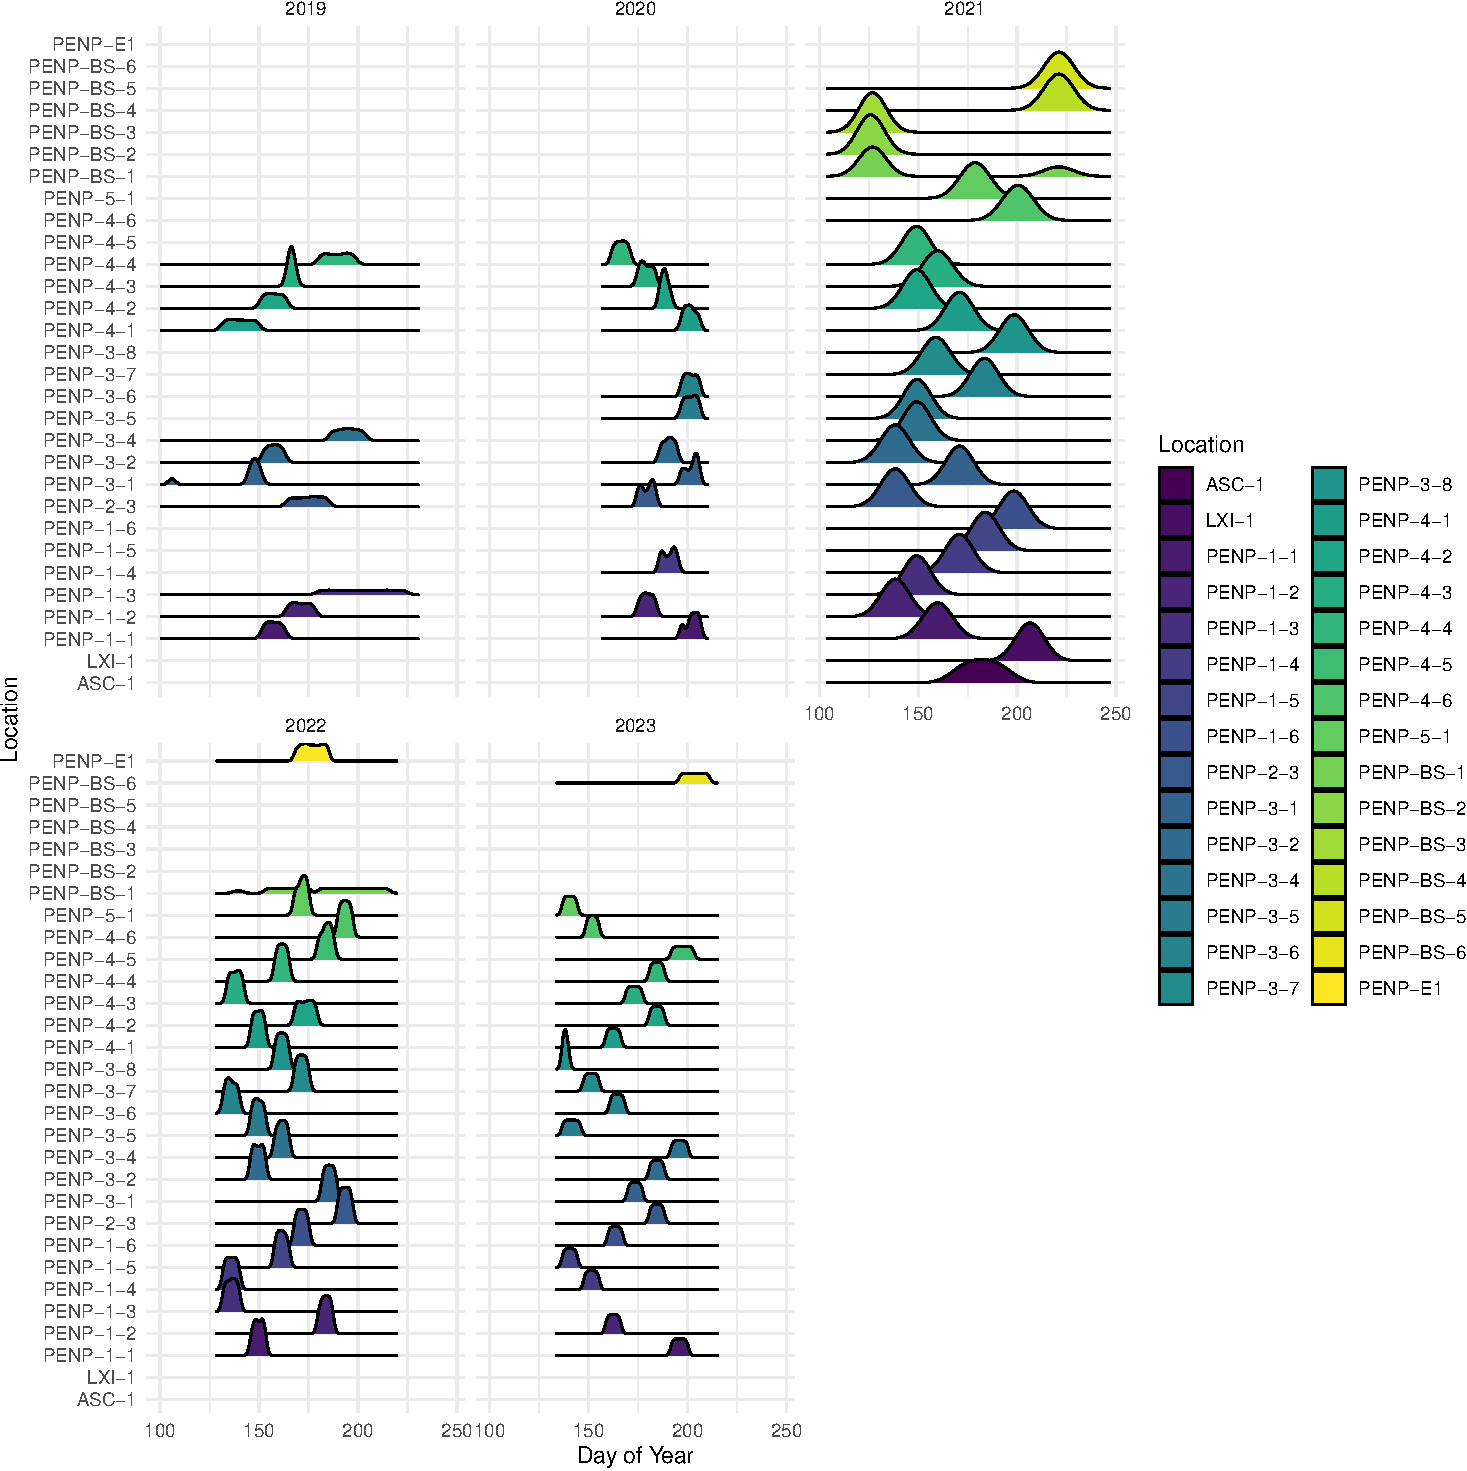
\includegraphics{peinp_files/figure-pdf/fig-recs-collect-1.pdf}

}

\end{figure}

\hypertarget{community-data-processing}{%
\subsection{Community data processing}\label{community-data-processing}}

The principal goal for data processing was to describe the acoustic
community of species heard at locations while choosing a large enough
subset of recordings for analyses. To ensure balanced replication, for
each location and year surveyed, four randomly selected recordings were
processed for 3-minutes between the hours of 4:00 AM - 7:59 AM ideally
on four separate dates (see Table~\ref{tbl-loc-repl}). Four recordings
will ensure that we have the minimum number of samples for a simple
occupancy analysis (Darryl I. MacKenzie et al.
(2002)\marginpar{\begin{footnotesize}\leavevmode\vadjust pre{\protect\hypertarget{ref-mackenzie2002estimating}{}}%
MacKenzie, Darryl I, James D Nichols, Gideon B Lachman, Sam Droege, J
Andrew Royle, and Catherine A Langtimm. 2002. {``Estimating Site
Occupancy Rates When Detection Probabilities Are Less Than One.''}
\emph{Ecology} 83 (8): 2248--55.\vspace{2mm}\par\end{footnotesize}}
and Darryl I. MacKenzie et al.
(2003)\marginpar{\begin{footnotesize}\leavevmode\vadjust pre{\protect\hypertarget{ref-imperfect-occu}{}}%
MacKenzie, Darryl I., James D. Nichols, James E. Hines, Melinda G.
Knutson, and Alan B. Franklin. 2003. {``ESTIMATING SITE OCCUPANCY,
COLONIZATION, AND LOCAL EXTINCTION WHEN a SPECIES IS DETECTED
IMPERFECTLY.''} \emph{Ecology} 84 (8): 2200--2207.
https://doi.org/\url{https://doi.org/10.1890/02-3090}.\vspace{2mm}\par\end{footnotesize}}).
Tags are made using count-removal (see Farnsworth et al.
(2002)\marginpar{\begin{footnotesize}\leavevmode\vadjust pre{\protect\hypertarget{ref-farnsworth2002removal}{}}%
Farnsworth, George L, Kenneth H Pollock, James D Nichols, Theodore R
Simons, James E Hines, and John R Sauer. 2002. {``A Removal Model for
Estimating Detection Probabilities from Point-Count Surveys.''}
\emph{The Auk} 119 (2): 414--25.\vspace{2mm}\par\end{footnotesize}},
Sólymos et al.
(2018)\marginpar{\begin{footnotesize}\leavevmode\vadjust pre{\protect\hypertarget{ref-time-removal}{}}%
Sólymos, Péter, Steven M. Matsuoka, Steven G. Cumming, Diana Stralberg,
Patricia Fontaine, Fiona K. A. Schmiegelow, Samantha J. Song, and Erin
M. Bayne. 2018. {``{Evaluating time-removal models for estimating
availability of boreal birds during point count surveys: Sample size
requirements and model complexity}.''} \emph{The Condor} 120 (4):
765--86. \url{https://doi.org/10.1650/CONDOR-18-32.1}.\vspace{2mm}\par\end{footnotesize}})
where tags are only made at the time of first detection of each
individual heard on the recordings. In case a species was overly
abundant a TMTT (`too many to tag') flag was used (see
Table~\ref{tbl-tmtt}). 1\% of the total tags were TMTT but were
subsequently converted to numeric using
\texttt{wildRtrax::wt\_replace\_tmtt}. We also verified that all tags
that were created were checked by a second observer (n = 67.46) to
ensure accuracy of detections (see Table~\ref{tbl-verified}). Amphibian
abundance was estimated at the time of first detection using the
\href{https://www.usgs.gov/centers/eesc/science/north-american-amphibian-monitoring-program}{North
American Amphibian Monitoring Program} with abundance of species being
estimated on the scale of ``calling intensity index'' (CI) of 1 - 3.
Mammals such as Red Squirrel, were also noted on the recordings. After
the data are processed in WildTrax, the
\href{https://abbiodiversity.github.io/wildRtrax/}{wildRtrax} package is
use to download the data into a standard format prepared for analysis.
The \texttt{wt\_download\_report} function downloads the data directly
to a R framework for easy manipulation (see
\href{https://abbiodiversity.github.io/wildRtrax/articles/apis.html}{wildRtrax
APIs}).

\begin{Shaded}
\begin{Highlighting}[]
\NormalTok{pei\_projects }\OtherTok{\textless{}{-}}\NormalTok{ wildRtrax}\SpecialCharTok{::}\FunctionTok{wt\_get\_download\_summary}\NormalTok{(}\AttributeTok{sensor =} \StringTok{\textquotesingle{}ARU\textquotesingle{}}\NormalTok{) }\SpecialCharTok{|\textgreater{}}
  \FunctionTok{filter}\NormalTok{(}\FunctionTok{grepl}\NormalTok{(}\StringTok{\textquotesingle{}\^{}Prince Edward Island National Park Forest Songbird\textquotesingle{}}\NormalTok{, project)) }\SpecialCharTok{|\textgreater{}}
  \FunctionTok{select}\NormalTok{(project\_id) }\SpecialCharTok{|\textgreater{}}
  \FunctionTok{pull}\NormalTok{()}

\NormalTok{pei\_main }\OtherTok{\textless{}{-}}
  \FunctionTok{map\_dfr}\NormalTok{(}
    \AttributeTok{.x =}\NormalTok{ pei\_projects,}
    \AttributeTok{.f =} \SpecialCharTok{\textasciitilde{}}\NormalTok{ wildRtrax}\SpecialCharTok{::}\FunctionTok{wt\_download\_report}\NormalTok{(}
      \AttributeTok{project\_id =}\NormalTok{ .x,}
      \AttributeTok{sensor\_id =} \StringTok{"ARU"}\NormalTok{,}
      \AttributeTok{weather\_cols =}\NormalTok{ T,}
      \AttributeTok{reports =} \StringTok{"main"}
\NormalTok{    )}
\NormalTok{  )}
\end{Highlighting}
\end{Shaded}

\hypertarget{tbl-loc-repl}{}
\begin{table}
\caption{\label{tbl-loc-repl}Example of tasks and unit replication for listening at PENP-1-1 }\tabularnewline

\centering
\begin{tabular}{l|r|l|l|r}
\hline
location & year & task\_duration & typ & n\\
\hline
PENP-1-1 & 2019 & 180s & Dawn & 6\\
\hline
PENP-1-1 & 2019 & 180s & Day & 7\\
\hline
PENP-1-1 & 2020 & 180s & Dawn & 9\\
\hline
PENP-1-1 & 2020 & 180s & Day & 2\\
\hline
PENP-1-1 & 2021 & 180s & Night & 4\\
\hline
PENP-1-1 & 2022 & 180s & Dawn & 4\\
\hline
PENP-1-1 & 2023 & 180s & Dawn & 4\\
\hline
\end{tabular}
\end{table}

\hypertarget{tbl-verified}{}
\begin{table}
\caption{\label{tbl-verified}Proportion of tags verified }\tabularnewline

\centering
\begin{tabular}{l|r|r}
\hline
Tag is verified & Count & Proportion\\
\hline
 & 137 & 1.32\\
\hline
f & 3239 & 31.22\\
\hline
t & 6998 & 67.46\\
\hline
\end{tabular}
\end{table}

\hypertarget{tbl-tmtt}{}
\begin{table}
\caption{\label{tbl-tmtt}TMTT tags }\tabularnewline

\centering
\begin{tabular}{l|l|l|l}
\hline
location & recording\_date\_time & species\_code & individual\_count\\
\hline
PENP-1-1 & 2019-06-01 05:25:00 & AMCR & TMTT\\
\hline
PENP-1-1 & 2019-06-01 05:25:00 & AMRE & TMTT\\
\hline
PENP-1-1 & 2019-06-02 06:24:00 & YEWA & TMTT\\
\hline
PENP-1-1 & 2019-06-02 06:24:00 & AMCR & TMTT\\
\hline
PENP-1-1 & 2019-06-02 06:24:00 & AMRE & TMTT\\
\hline
PENP-1-1 & 2019-06-04 07:23:00 & AMRE & TMTT\\
\hline
\end{tabular}
\end{table}

\hypertarget{visual-scanning}{%
\subsection{Visual scanning}\label{visual-scanning}}

Visual scanning is the concept of visually examining spectrograms in
order to find a signal within an audio recording. Visual scanning can be
a useful processing method allowing trained users to process recordings
much faster than traditional listening. It has been used for detecting
different taxa (amphibians: Cameron et al.
(2020)\marginpar{\begin{footnotesize}\leavevmode\vadjust pre{\protect\hypertarget{ref-vis-scan-amphs}{}}%
Cameron, J., A. Crosby, C. Paszkowski, and E. Bayne. 2020. {``Visual
Spectrogram Scanning Paired with an Observation--Confirmation Occupancy
Model Improves the Efficiency and Accuracy of Bioacoustic Anuran
Data.''} \emph{Canadian Journal of Zoology} 98 (11): 733--42.
\url{https://doi.org/10.1139/cjz-2020-0103}.\vspace{2mm}\par\end{footnotesize}},
mammals: Garland et al.
(2020)\marginpar{\begin{footnotesize}\leavevmode\vadjust pre{\protect\hypertarget{ref-aru-vs-cams-wolves}{}}%
Garland, Laura, Andrew Crosby, Richard Hedley, Stan Boutin, and Erin
Bayne. 2020. {``Acoustic Vs. Photographic Monitoring of Gray Wolves
({Canis lupus}): A Methodological Comparison of Two Passive Monitoring
Techniques.''} \emph{Canadian Journal of Zoology} 98 (3): 219--28.
\url{https://doi.org/10.1139/cjz-2019-0081}.\vspace{2mm}\par\end{footnotesize}})
with comparable biological metrics, as well as helping to maximize
species detection in large acoustic monitoring data sets (Ware et al.
(2023)\marginpar{\begin{footnotesize}\leavevmode\vadjust pre{\protect\hypertarget{ref-all-the-scans}{}}%
Ware, Lena, C. Lisa Mahon, Logan McLeod, and Jean-François Jetté. 2023.
{``Artificial Intelligence (BirdNET) Supplements Manual Methods to
Maximize Bird Species Richness from Acoustic Data Sets Generated from
Regional Monitoring.''} \emph{Canadian Journal of Zoology} 101 (12):
1031--51. \url{https://doi.org/10.1139/cjz-2023-0044}.\vspace{2mm}\par\end{footnotesize}}).
WildTrax's project settings and dynamic spectrogram settings in the
processing interface allow users to upload many recordings, while also
allowing frequency-limited or time-limited spectrograms. These changes
are easily made by adjusting project settings in WildTrax (see
Figure~\ref{fig-project-dynamic}).

\begin{figure}

{\centering 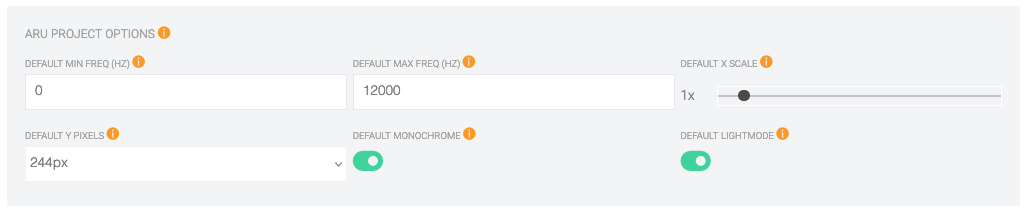
\includegraphics{project-dynamic.png}

}

\caption{\label{fig-project-dynamic}Dynamic spectrogram and project
settings in WildTrax}

\end{figure}

In order to determine presence of Bank Swallow (BANS) at
\texttt{PENP-BS-*} site, visual scanning was employed to identify the
time of first detection of the species on recordings at these locations.
A total of 630 recordings were visually scanned for BANS. Tags were made
at the time of first detection in each minute interval.

\hypertarget{automated-recognition}{%
\subsection{Automated recognition}\label{automated-recognition}}

Automated recognition is a well-known process to help detect rare and
elusive species (Knight and Bayne
(2019)\marginpar{\begin{footnotesize}\leavevmode\vadjust pre{\protect\hypertarget{ref-knight2019classification}{}}%
Knight, Elly C, and Erin M Bayne. 2019. {``Classification Threshold and
Training Data Affect the Quality and Utility of Focal Species Data
Processed with Automated Audio-Recognition Software.''}
\emph{Bioacoustics} 28 (6): 539--54.\vspace{2mm}\par\end{footnotesize}}.
Shonfield, Heemskerk, and Bayne
(2018)\marginpar{\begin{footnotesize}\leavevmode\vadjust pre{\protect\hypertarget{ref-shonfield2018utility}{}}%
Shonfield, Julia, Sarah Heemskerk, and Erin M Bayne. 2018. {``Utility of
Automated Species Recognition for Acoustic Monitoring of Owls.''}
\emph{Journal of Raptor Research} 52 (1): 42--55.\vspace{2mm}\par\end{footnotesize}})
as well as species that may have a low detectability by collecting large
data sets. In order to determine We constructed a recognizer for Eastern
Wood-Pewee (EAWP) and used three previously constructed Wildlife
Acoustics SongScope recognizers for Olive-sided Flycatcher (OSFL), Rusty
Blackbird (RUBL) and Canada Warbler (CAWA) to detect for the presence of
these species in the 2019 data set. All recognizers are freely available
on WildTrax under Methods and Protocols \textgreater{}
\href{https://wildtrax.ca/resources/methods-protocols/automated-recognizers/}{Automated
Recognizers}. Hits were verified and true positives for presence at each
location (recording where the species was first positively detected)
were uploaded to WildTrax via the \texttt{wt\_songscope\_tags} function
in \texttt{wildRtrax}.

\hypertarget{analyses}{%
\subsection{Analyses}\label{analyses}}

Species richness, diversity and occupancy were calculated using the 21
forest songbird monitoring locations (\texttt{PENP-}). We calculated
species richness as distinct species found at each location and year
surveyed (see Figure~\ref{fig-spp-rich-locs}), omitting species using
\texttt{wildRtrax::wt\_tidy\_species()} for abiotic, amphibians,
unknowns and insects. To determine if there were any changes to species
diversity, we used Shannon's diversity index over years using
\texttt{vegan::diversity} (see Figure~\ref{fig-shannon}).

For testing species occupancy, we selected locations with a minimum of
four dawn visits for each year across all five years, focusing on forest
obligate species for ecological relevance (see
Table~\ref{tbl-bird-guilds}). Utilizing a single-season single-species
occupancy model from Darryl I. MacKenzie et al.
(2002)\marginpar{\begin{footnotesize}\leavevmode\vadjust pre{\protect\hypertarget{ref-mackenzie2002estimating}{}}%
MacKenzie, Darryl I, James D Nichols, Gideon B Lachman, Sam Droege, J
Andrew Royle, and Catherine A Langtimm. 2002. {``Estimating Site
Occupancy Rates When Detection Probabilities Are Less Than One.''}
\emph{Ecology} 83 (8): 2248--55.\vspace{2mm}\par\end{footnotesize}},
we calculated the predicted occupancy of species at all locations
surveyed in each year across years. Site-specific covariates included
the distance to ocean edge (in meters) and the proportional area of each
cover type from the
\href{https://data.princeedwardisland.ca/Environment-and-Food/OD0144-Corporate-Landuse-Inventory-2010/tc7z-7rpy}{Prince
Edward Island 2010 Corporate Land Use Inventory} at 150 meter radius
surrounding the ARU categorized into anthropogenic (pavement, soy), open
(grass, sand dune, bare soil), deciduous (red maple, white birch, alder,
poplar) and conifer (white spruce, black spruce, balsam fir).
Observation covariates incorporated day of the year, hour, observer, and
a quadratic term for both day of year (\(doy^{2}\)) and hour
(\(hr^{2}\)). See Table~\ref{tbl-obvs-and-covs} for more information.
Despite variations in processing methodology between 2019 - 2020 (1SPM -
species-individual detected per minute, i.e.~repeat sampling each minute
for 3 minute) and subsequent years (2021 - 2023; 1SPT), we maintained
consistency by exclusively utilizing the time to the first detection of
individuals from the 1SPM recordings. Model predictions were generated,
with goodness-of-fit testing using methods from Darryl I. MacKenzie and
Bailey
(2004)\marginpar{\begin{footnotesize}\leavevmode\vadjust pre{\protect\hypertarget{ref-occu-fit}{}}%
MacKenzie, Darryl I., and Larissa L. Bailey. 2004. {``Assessing the Fit
of Site-Occupancy Models.''} \emph{Journal of Agricultural, Biological,
and Environmental Statistics} 9 (3): 300--318.
\url{http://www.jstor.org/stable/1400484}.\vspace{2mm}\par\end{footnotesize}}
and the best model selected based on AIC and through
\texttt{MuMIn::dregde}, \texttt{MuMIn::get.models} and
\texttt{MuMIn::model.sel}. If more than one model existed, the average
model was used using \texttt{MuMIn::model.avg}. The final predictions
were then made and plotted over years and sorted by nesting guilds of
species into conifer, deciduous, treed / shrubby and open.

\begin{center}\rule{0.5\linewidth}{0.5pt}\end{center}

\hypertarget{results}{%
\section{Results}\label{results}}

\hypertarget{species-richness}{%
\subsection{Species richness}\label{species-richness}}

A total of 100 species were found across the five years.
Figure~\ref{fig-spp-rich-locs} describes the relationship of species
richness across each location and survey year with
Figure~\ref{fig-spp-rich-annual} showing the relationship between
species richness and survey effort.

\begin{figure}

\sidecaption{\label{fig-spp-rich-locs}Species richness at forest
monitoring locations across years}

{\centering 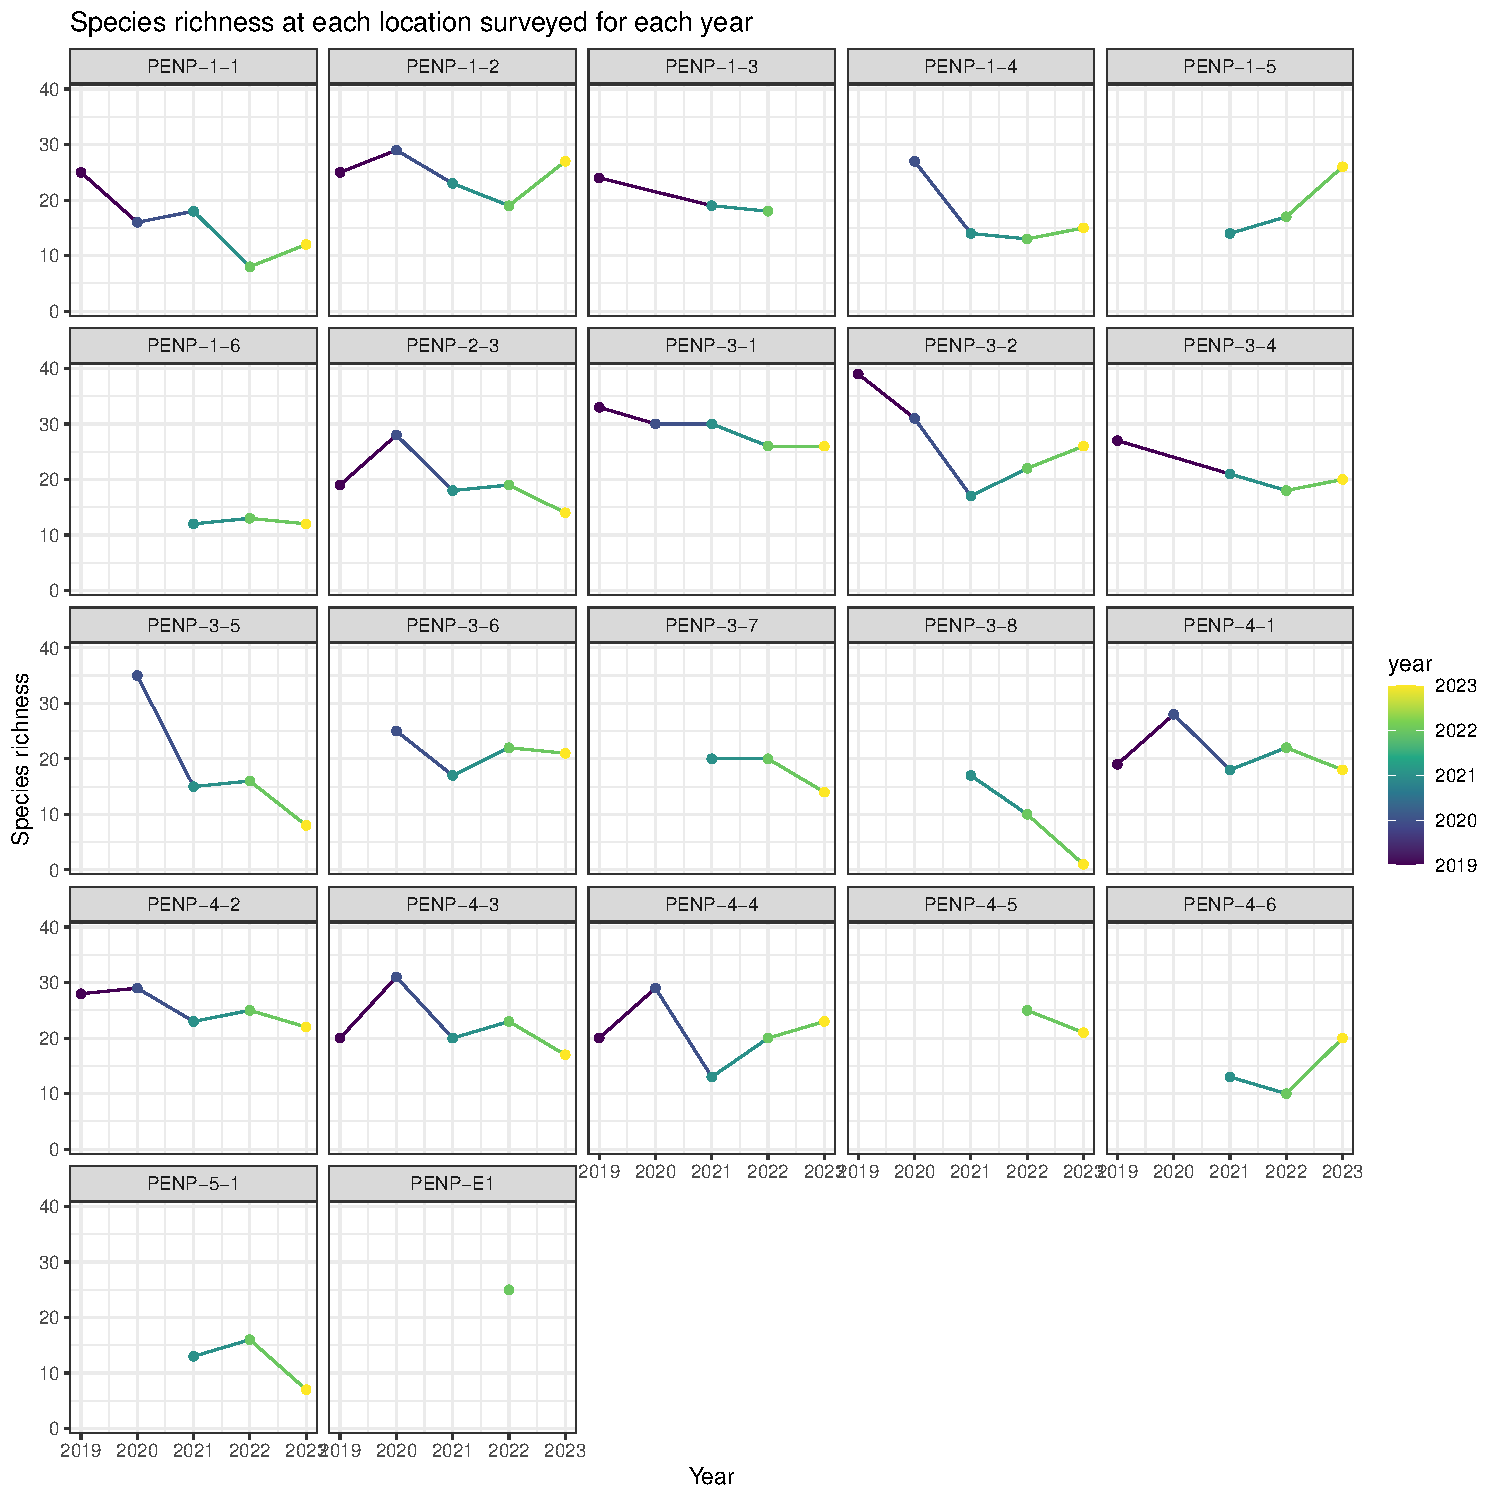
\includegraphics{peinp_files/figure-pdf/fig-spp-rich-locs-1.pdf}

}

\end{figure}

\begin{figure}

\sidecaption{\label{fig-spp-rich-annual}Species richness at forest
monitoring locations across years considering sampling effort}

{\centering 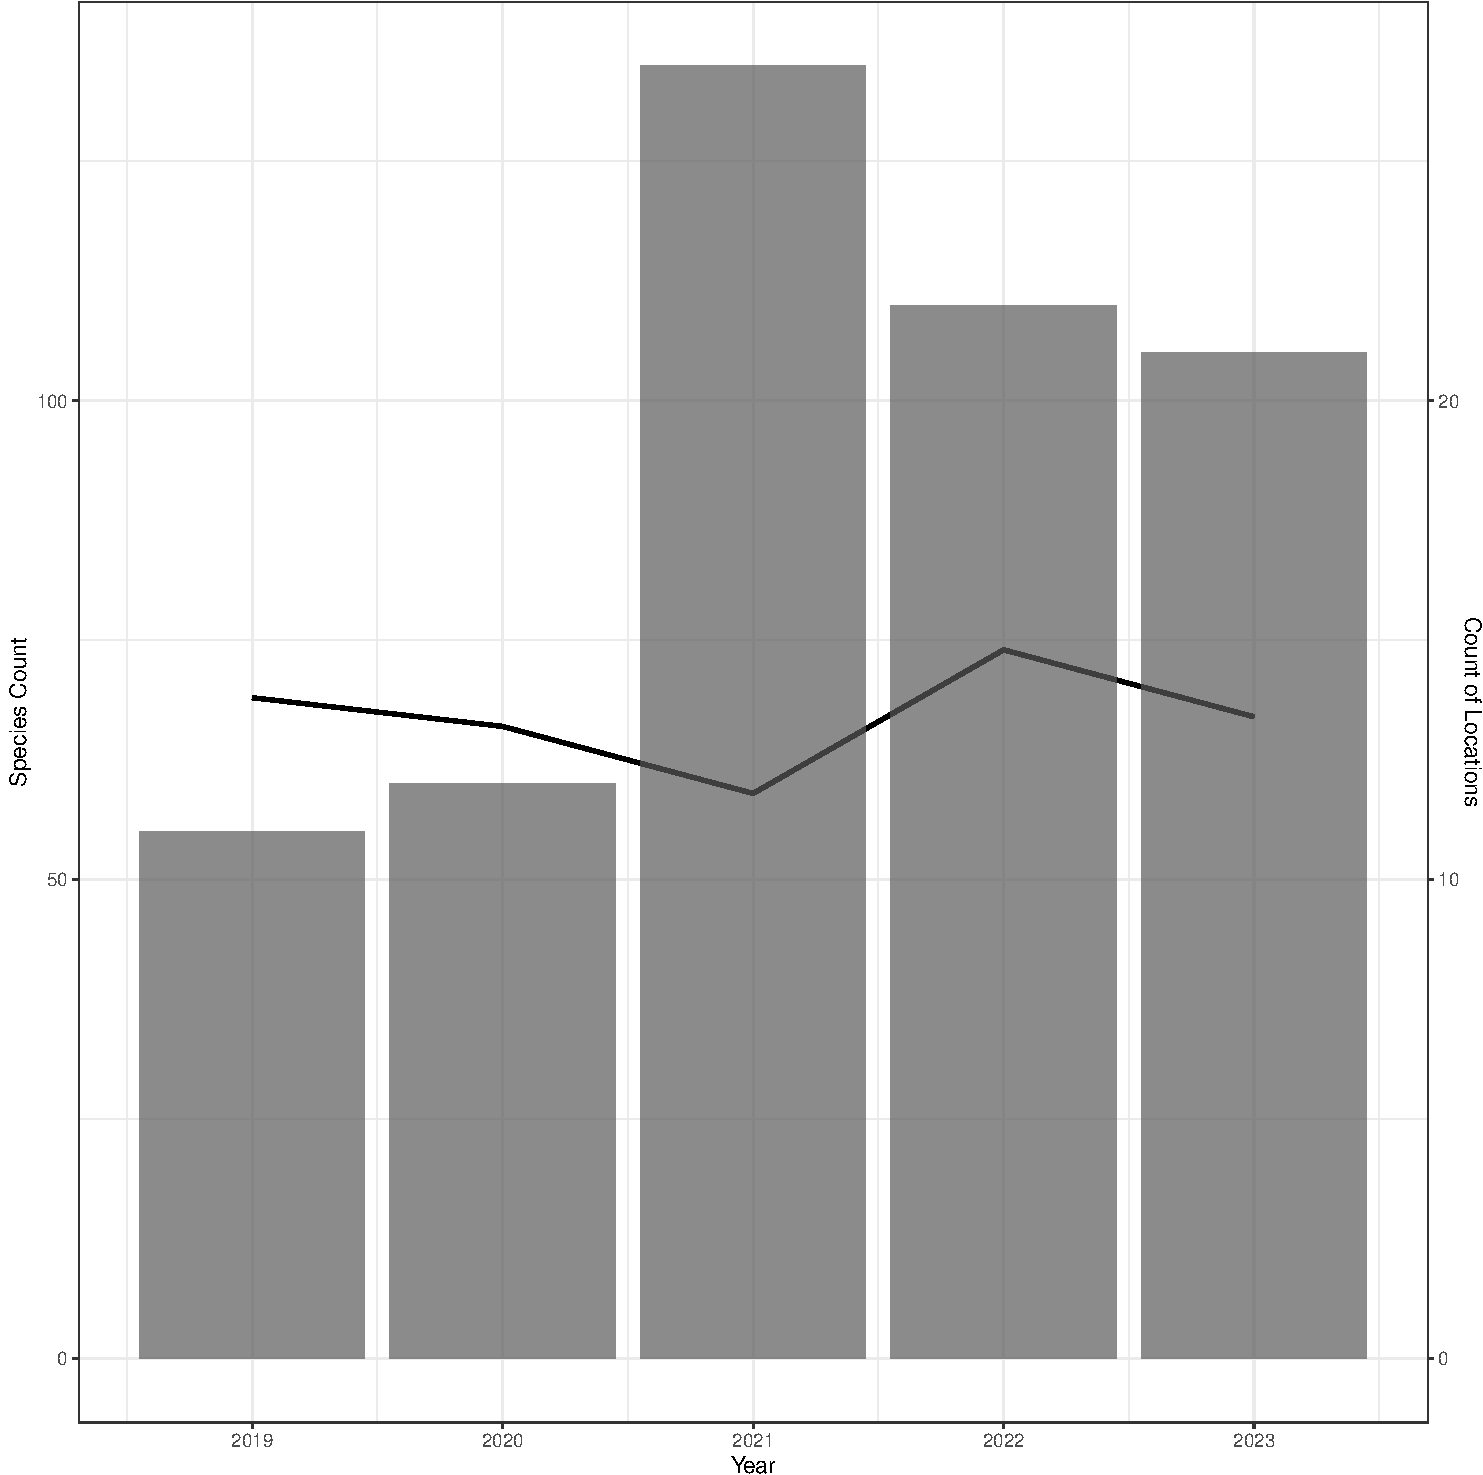
\includegraphics{peinp_files/figure-pdf/fig-spp-rich-annual-1.pdf}

}

\end{figure}

\hypertarget{tbl-bird-guilds}{}
\begin{table}
\caption{\label{tbl-bird-guilds}Bird guilds. For nesting habitat; Ag = Agricultural, Be = Beach, Bo =
Bog, CW = Coniferous Woodlands, ES = Early Successional, MW = Mixed
Woodlands, OW = Open Woodlands, TSS = Treed/Shrubby Swamp, Ur = Urban.
Species from CW, MW, OW, TSS were used for analysis. }\tabularnewline

\centering
\begin{tabular}{l|l|l|l|l|l|l|l}
\hline
species\_common\_name & general\_type & migration & feeding & breeding\_substrate & foraging\_type & substrate\_nesting & habitat\_nesting\\
\hline
Alder Flycatcher & S & NM & In & Air & Sal & Sh & TSS\\
\hline
American Redstart & NA & NA & NA & NA & NA & NA & MW\\
\hline
Baltimore Oriole & NA & NA & NA & NA & NA & NA & OW\\
\hline
Bay-breasted Warbler & NA & NA & NA & NA & NA & NA & CW\\
\hline
Black-and-white Warbler & NA & NA & NA & NA & NA & NA & MW\\
\hline
Black-backed Woodpecker & S & R & In & Ba & Sca & Sn & CW\\
\hline
Black-throated Blue Warbler & NA & NA & NA & NA & NA & NA & MW\\
\hline
Black-throated Green Warbler & NA & NA & NA & NA & NA & NA & CW\\
\hline
Blackburnian Warbler & NA & NA & NA & NA & NA & NA & CW\\
\hline
Blackpoll Warbler & NA & NA & NA & NA & NA & NA & CW\\
\hline
Blue Jay & G & NA & NA & NA & NA & NA & OW\\
\hline
Blue-headed Vireo & S & SDM & In & LCS & Gl & CT & MW\\
\hline
Boreal Chickadee & S & R & In & LCS & Gl & Sn & CW\\
\hline
Brown Creeper & NA & NA & NA & NA & NA & NA & CW\\
\hline
Canada Jay & G & R & Om & UC & Fo & CT & CW\\
\hline
Canada Warbler & NA & NA & NA & NA & NA & NA & MW\\
\hline
Cape May Warbler & NA & NA & NA & NA & NA & NA & CW\\
\hline
Chestnut-sided Warbler & NA & NA & NA & NA & NA & NA & MW\\
\hline
Chipping Sparrow & G & SDM & Om & Gr & Fo & CT & OW\\
\hline
Common Nighthawk & S & NM & In & Air & Scr & Gr & OW\\
\hline
Dark-eyed Junco & G & SDM & Om & Gr & Fo & Gr & CW\\
\hline
Downy Woodpecker & G & NA & NA & NA & NA & NA & MW\\
\hline
Eastern Wood-Pewee & S & NA & NA & NA & NA & NA & OW\\
\hline
Fox Sparrow & G & SDM & Om & Gr & Fo & Gr & OW\\
\hline
Golden-crowned Kinglet & S & NA & NA & NA & NA & NA & CW\\
\hline
Gray Catbird & S & NA & NA & NA & NA & NA & MW\\
\hline
Hairy Woodpecker & NA & NA & NA & NA & NA & NA & MW\\
\hline
Hermit Thrush & S & SDM & In & Gr & Gl & Gr & CW\\
\hline
Lincoln's Sparrow & NA & NA & NA & NA & NA & NA & TSS\\
\hline
Magnolia Warbler & NA & NA & NA & NA & NA & NA & MW\\
\hline
Mountain Bluebird & S & SDM & In & Gr & Gl & Sn & OW\\
\hline
Mourning Warbler & NA & NA & NA & NA & NA & NA & MW\\
\hline
Northern Flicker & S & SDM & In & Gr & Gl & Sn & MW\\
\hline
Northern Parula & NA & NA & NA & NA & NA & NA & OW\\
\hline
Orange-crowned Warbler & S & SDM & In & LCS & Gl & Gr & OW\\
\hline
Philadelphia Vireo & NA & NA & NA & NA & NA & NA & MW\\
\hline
Pileated Woodpecker & S & R & In & Ba & Ex & Sn & MW\\
\hline
Pine Warbler & NA & NA & NA & NA & NA & NA & CW\\
\hline
Red-eyed Vireo & NA & NA & NA & NA & NA & NA & MW\\
\hline
Ruby-crowned Kinglet & S & SDM & In & UC & Gl & CT & CW\\
\hline
Ruffed Grouse & G & R & Om & Gr & Fo & Gr & MW\\
\hline
Rusty Blackbird & NA & NA & NA & NA & NA & NA & TSS\\
\hline
Swainson's Thrush & G & NM & Om & Gr & Fo & CT & MW\\
\hline
Veery & NA & NA & NA & NA & NA & NA & MW\\
\hline
Warbling Vireo & NA & NA & NA & NA & NA & NA & MW\\
\hline
Western Wood-Pewee & S & NM & In & Air & Sal & CT & OW\\
\hline
Yellow-bellied Sapsucker & G & SDM & Om & Ba & Ex & DT & MW\\
\hline
Yellow-rumped Warbler & S & SDM & In & LCS & Gl & CT & CW\\
\hline
\end{tabular}
\end{table}

\begin{figure}

\sidecaption{\label{fig-spp-activity}Seasonal detection activity of most
commonly detected forest species}

{\centering 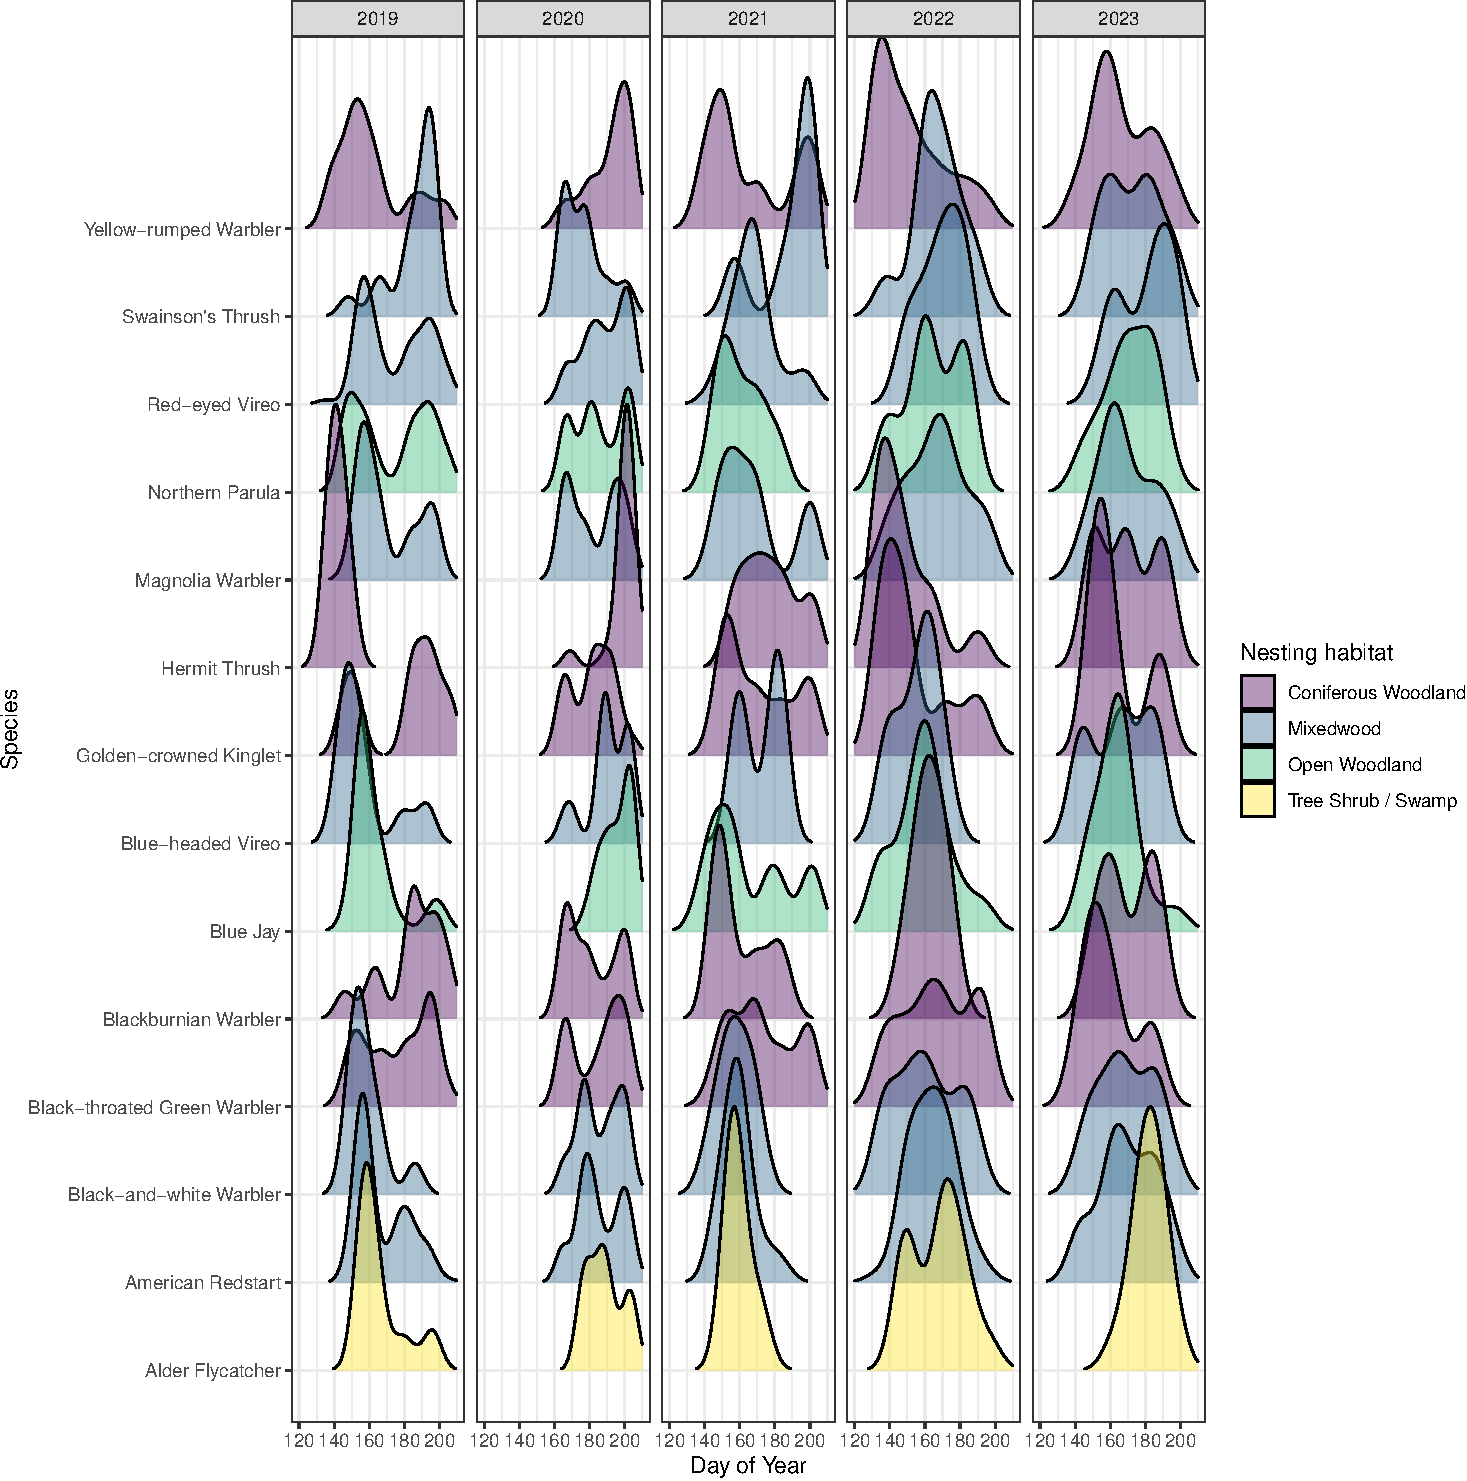
\includegraphics{peinp_files/figure-pdf/fig-spp-activity-1.pdf}

}

\end{figure}

\hypertarget{species-diversity}{%
\subsection{Species diversity}\label{species-diversity}}

Shannon's diversity was stable based on results. (see
Figure~\ref{fig-shannon}.)

\begin{figure}

{\centering 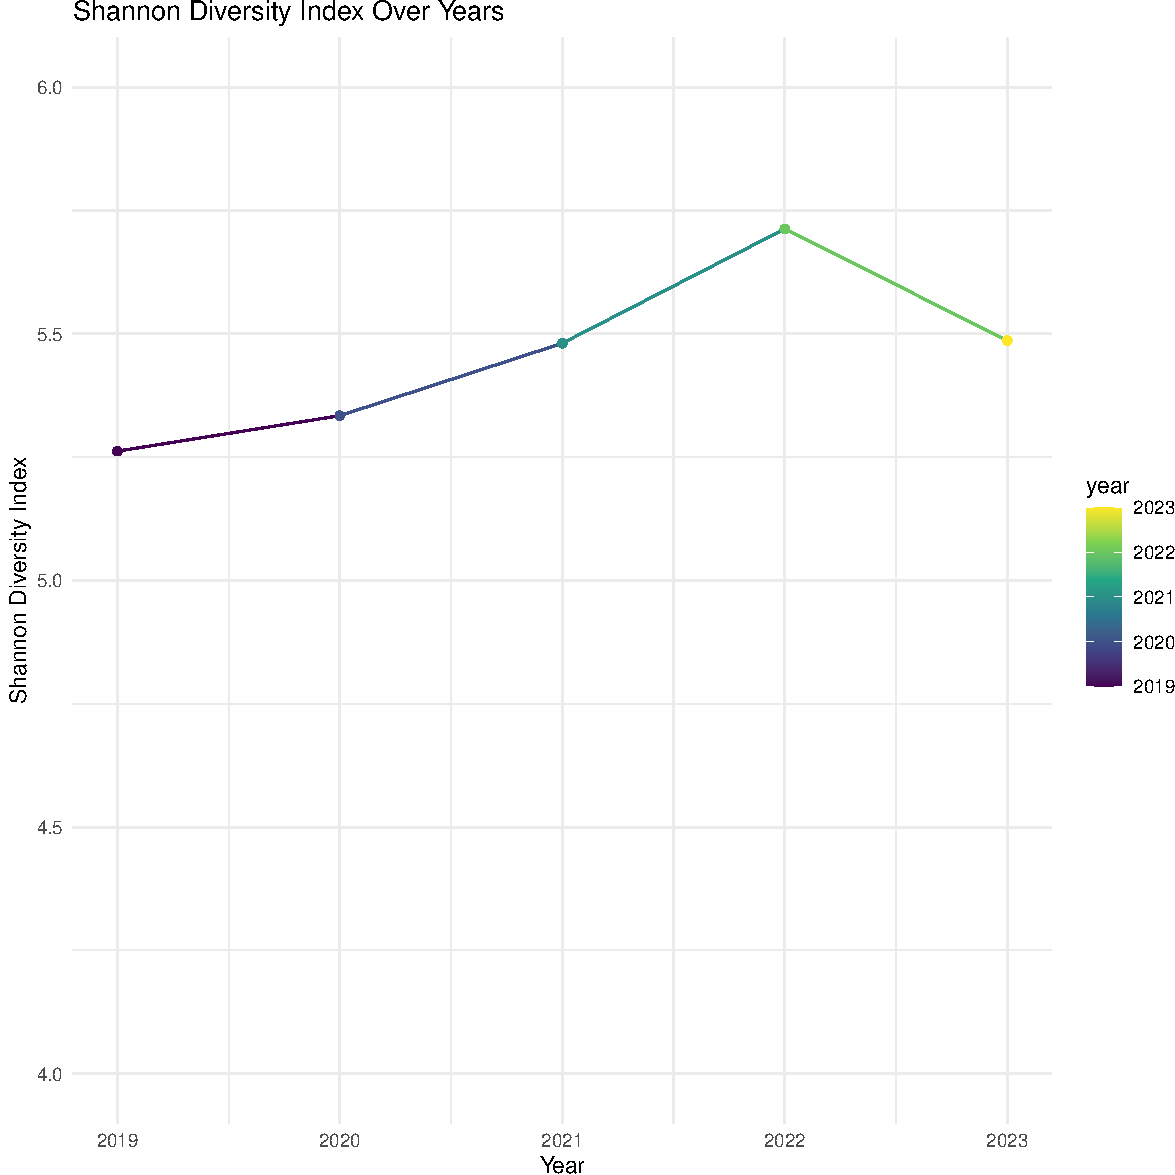
\includegraphics{peinp_files/figure-pdf/fig-shannon-1.pdf}

}

\caption{\label{fig-shannon}Shannon's diversity across years for all
locations surveyed.}

\end{figure}

\hypertarget{species-occupancy}{%
\subsection{Species occupancy}\label{species-occupancy}}

We selected \texttt{20} species to represent the forest songbird
community into 4 separate habitat nesting guilds (see
Table~\ref{tbl-bird-guilds}): conifer
(Figure~\ref{fig-spp-occ-conifer}), deciduous
(Figure~\ref{fig-spp-occ-decid}), treed / shrubby
(Figure~\ref{fig-spp-occ-tss}) and open (Figure~\ref{fig-spp-occ-open}).
Analysis of species occupancy revealed diverse and varied changes across
these species. Analytically, many models were singular, and a few
exhibited overdispersion (indicated by \emph{c-hat} in
\textbf{?@tbl-c-hat}), likely due to low detections or a limited sample
size of spatial locations. Ubiquitous species such as Yed-eyed Vireo,
Yellow-rumped Warbler, Magnolia Warbler and Northern Parula,
demonstrated stable site occupancy across the years. Generalist species
or those capable of capitalizing on utilizing mixed habitats,
exemplified by the Northern Parula, also maintained consistent occupancy
levels. The occurrence of Hurricane Fiona in 2023 led to notable
breakpoints in the occupancy of certain species: coniferous species,
including the Black-throated Green Warbler, Black-throated Blue Warbler,
Blackburnian Warbler, Golden-crowned Kinglet, and Mourning Warbler,
experienced declines. Conversely, increases were observed in guilds of
species that favor more open or shrubby habitats, such as the Alder
Flycatcher and American Redstart. Thrushes (American Robin, Swainson's
Thrush, Hermit Thrush) had notably wavering occupancy throughout the
years.

\begin{figure}

{\centering 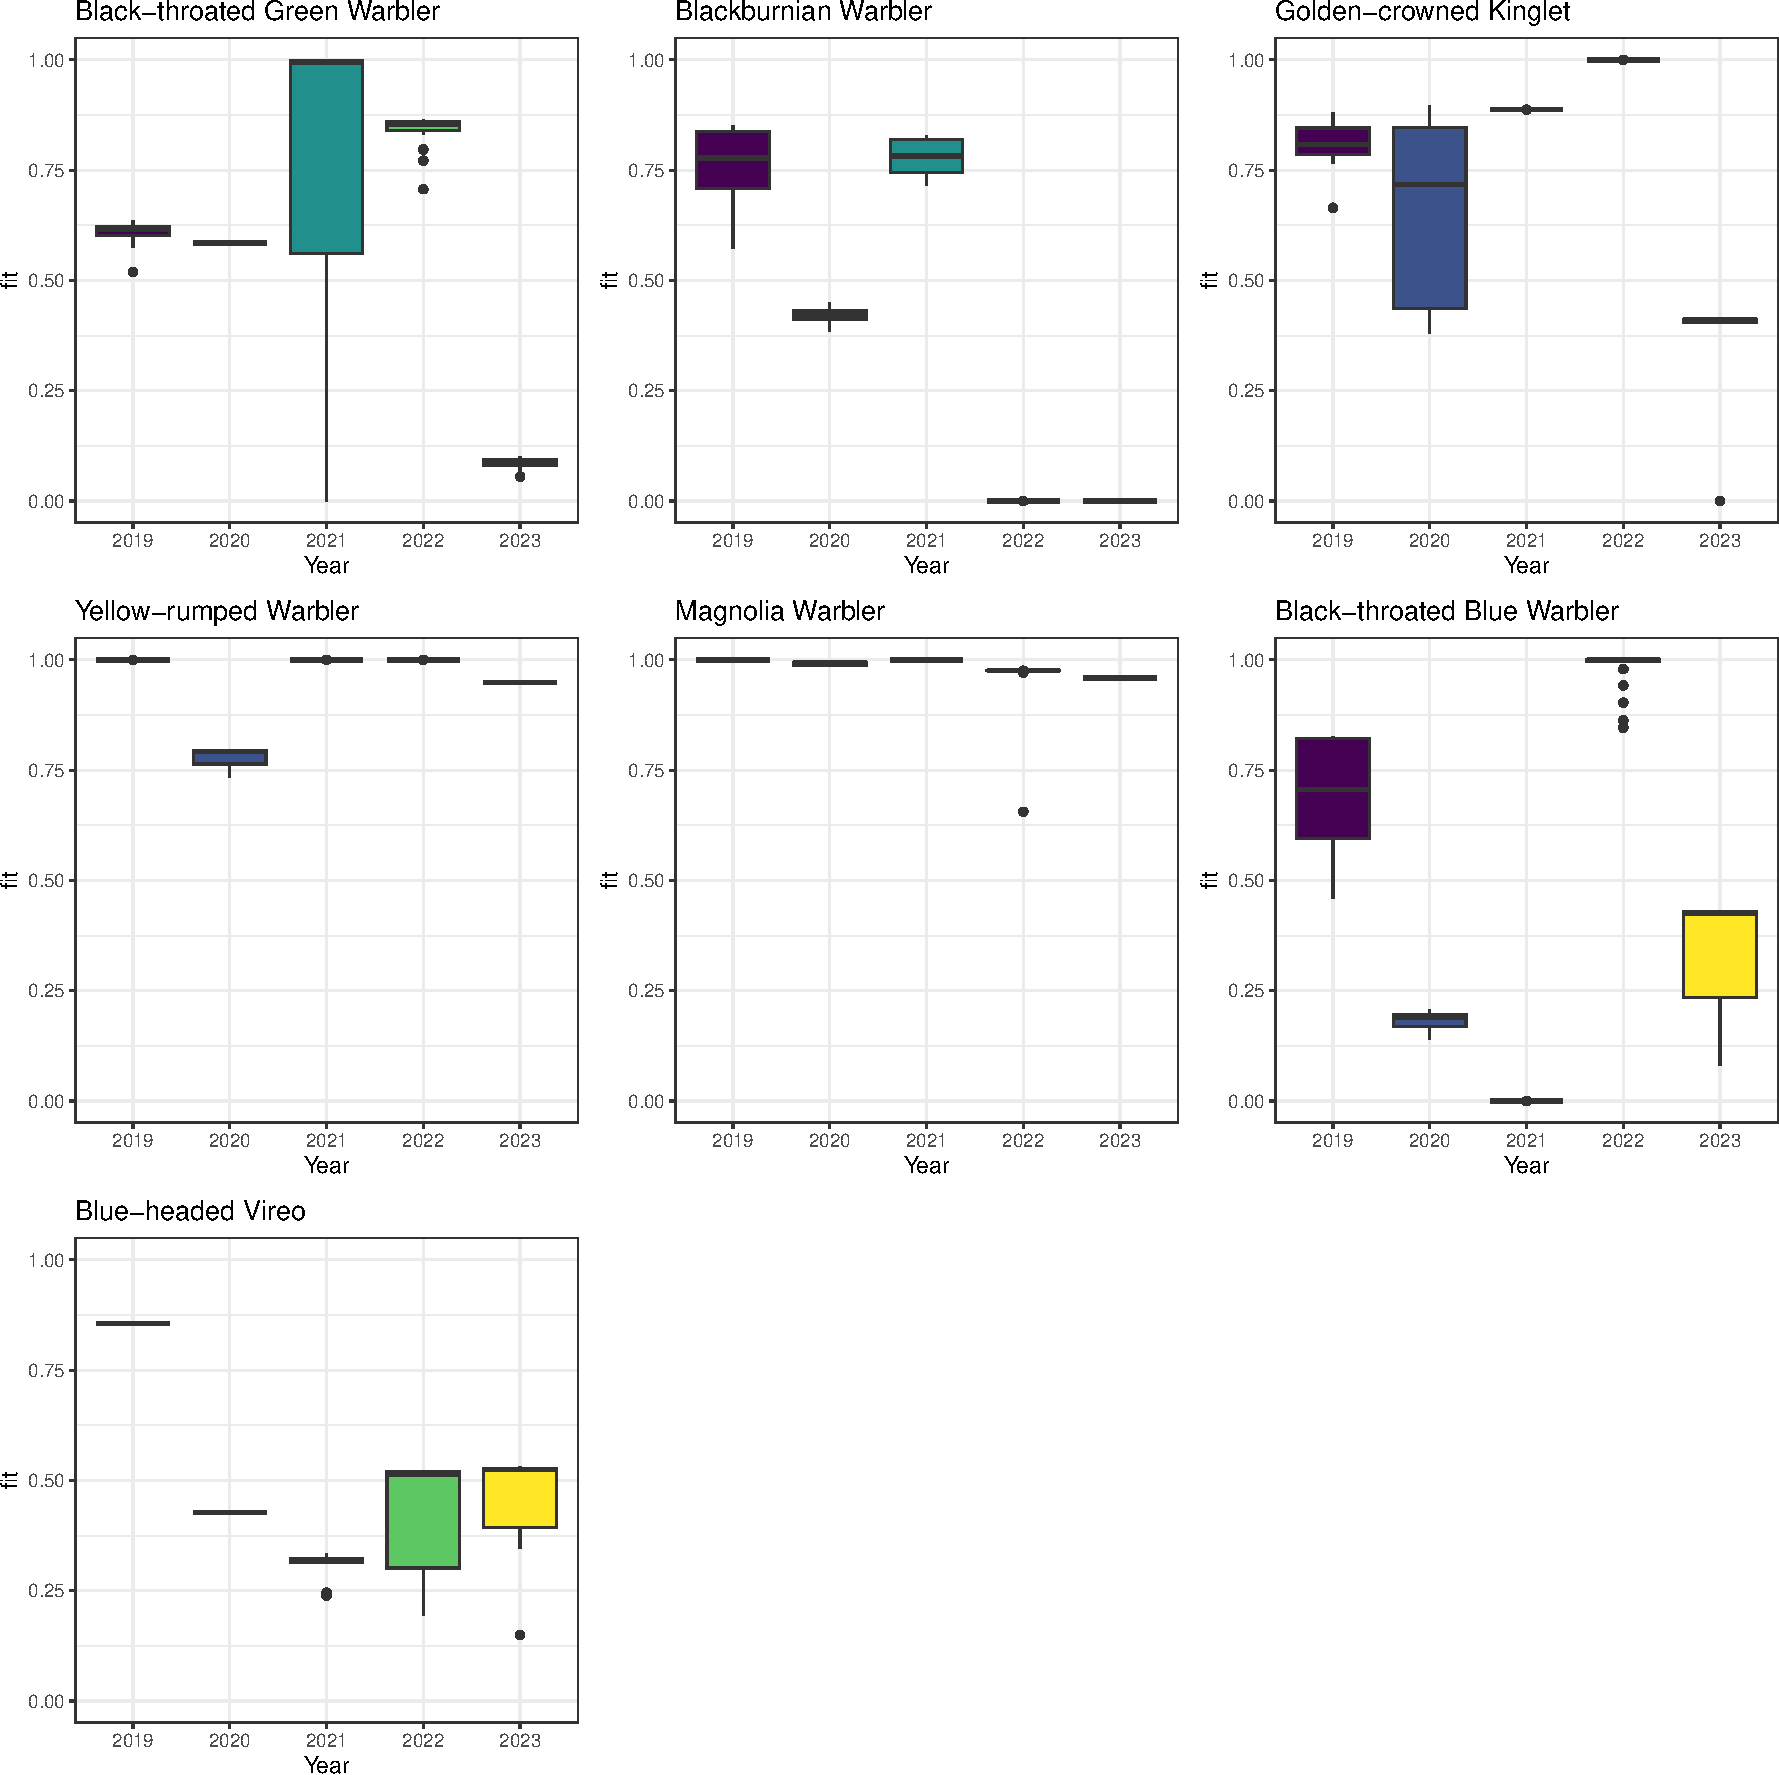
\includegraphics{peinp_files/figure-pdf/fig-spp-occ-conifer-1.pdf}

}

\caption{\label{fig-spp-occ-conifer}Predicted single-season occupancy of
forest species (Habitat nesting = Conifer) within Prince Edward Island
National Park. The data represents the average species occupancy across
all surveyed locations for each respective year.}

\end{figure}

\begin{figure}

{\centering 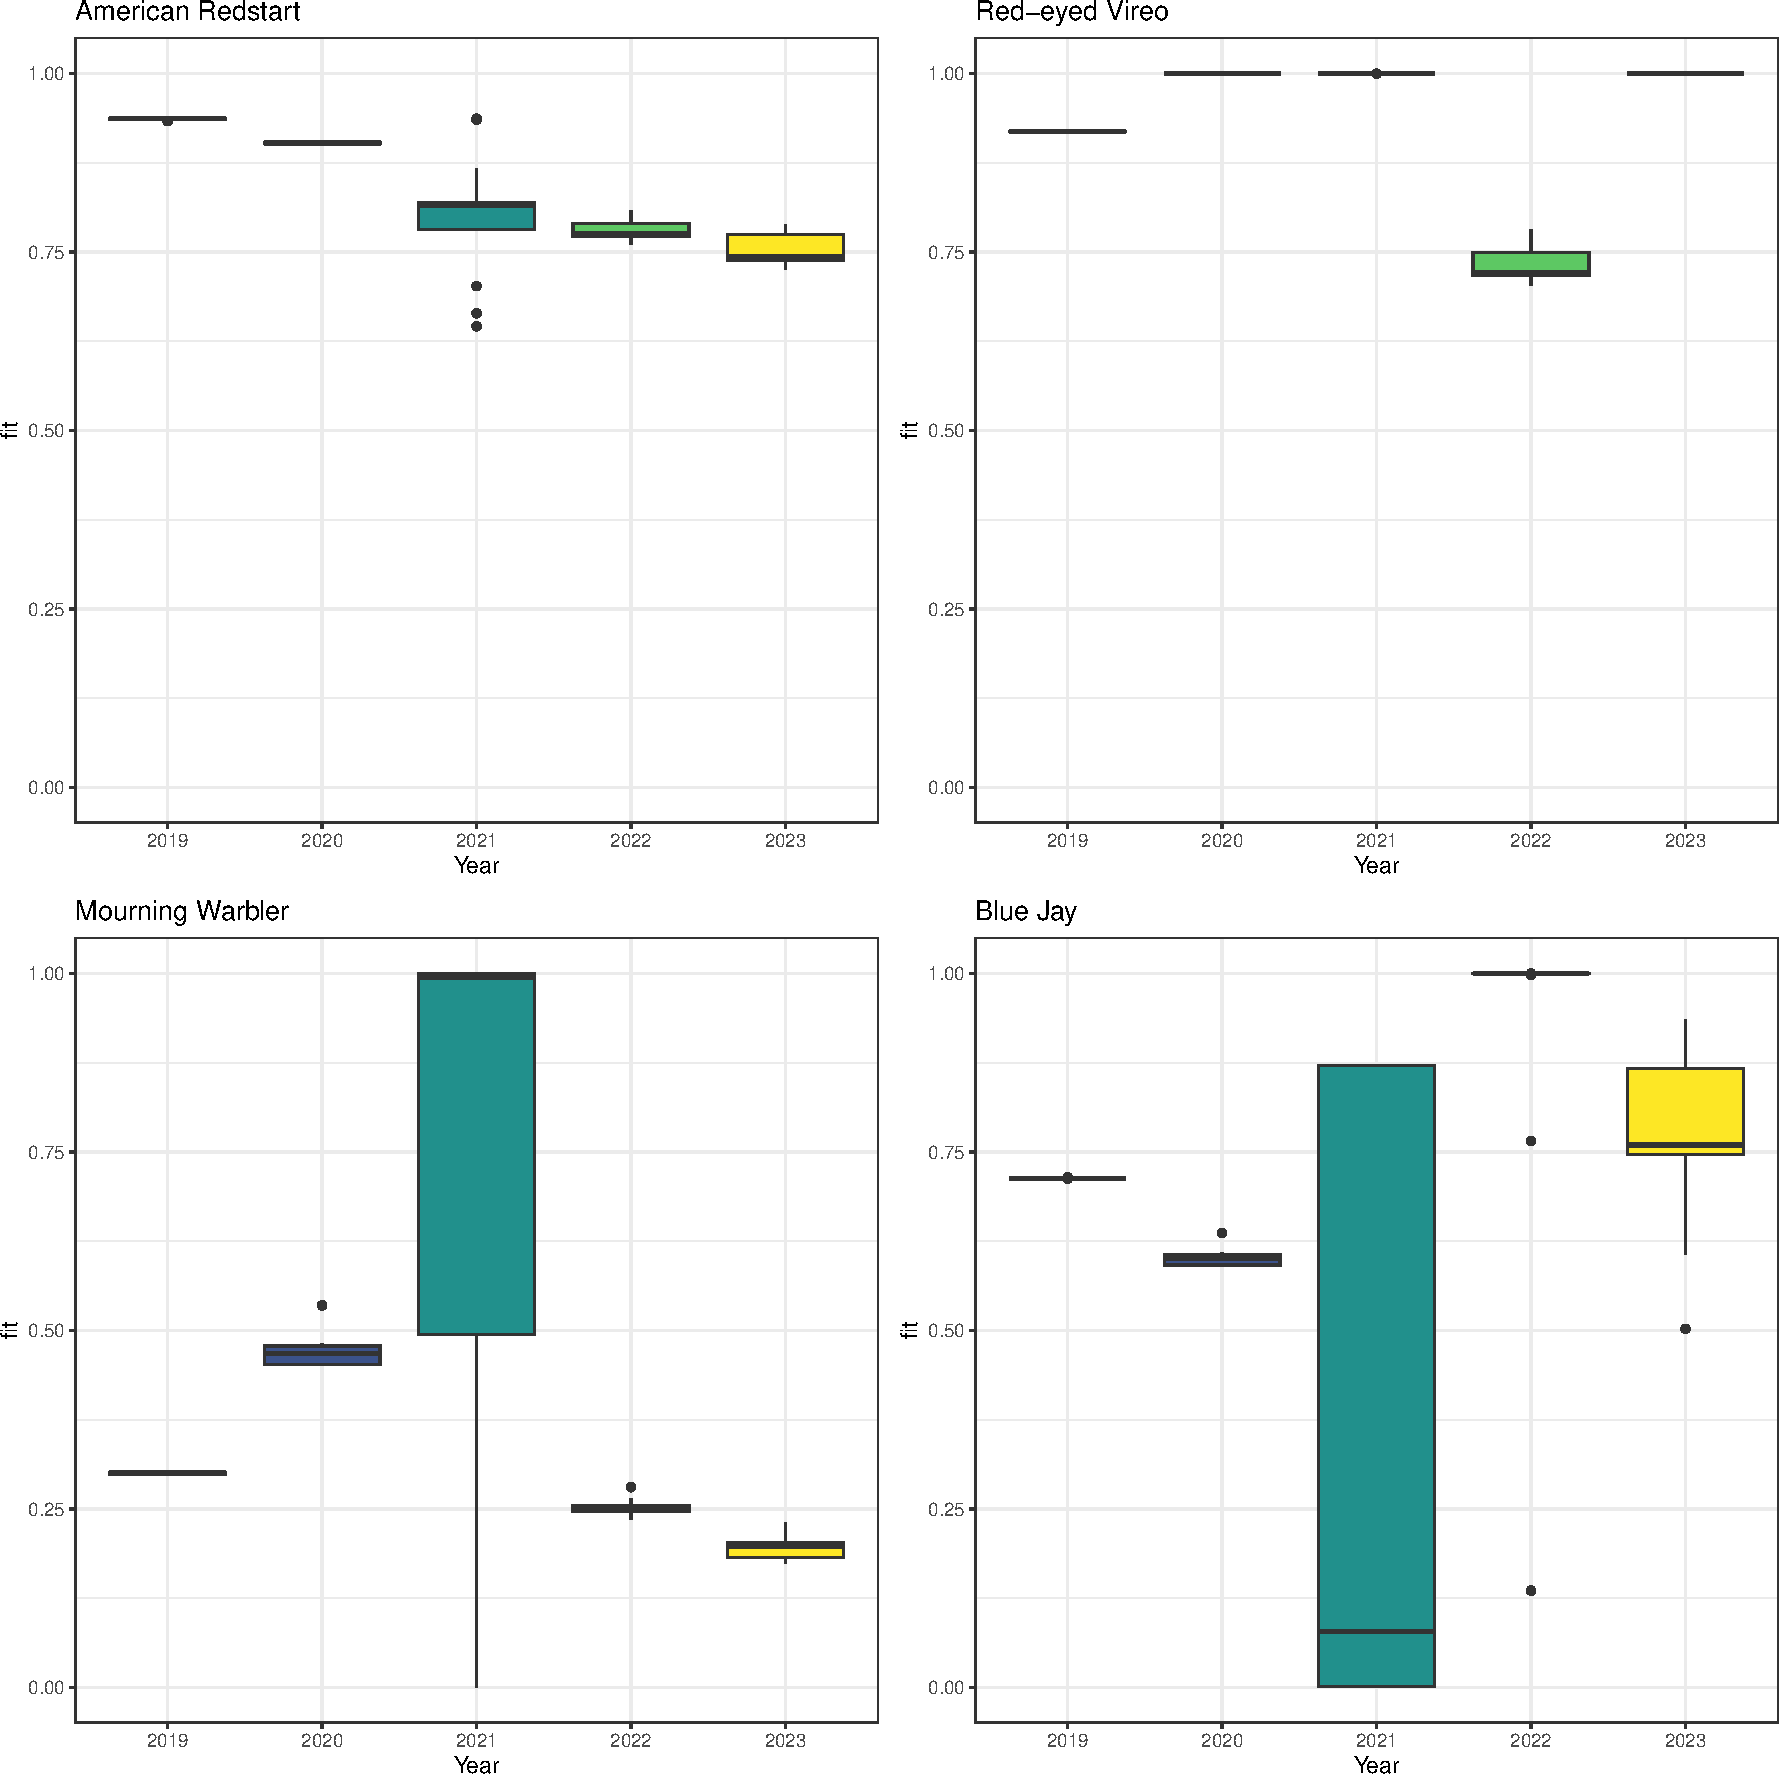
\includegraphics{peinp_files/figure-pdf/fig-spp-occ-decid-1.pdf}

}

\caption{\label{fig-spp-occ-decid}Predicted single-season occupancy of
forest species (Habitat nesting = Deciduous) within Prince Edward Island
National Park. The data represents the average species occupancy across
all surveyed locations for each respective year.}

\end{figure}

\begin{figure}

{\centering 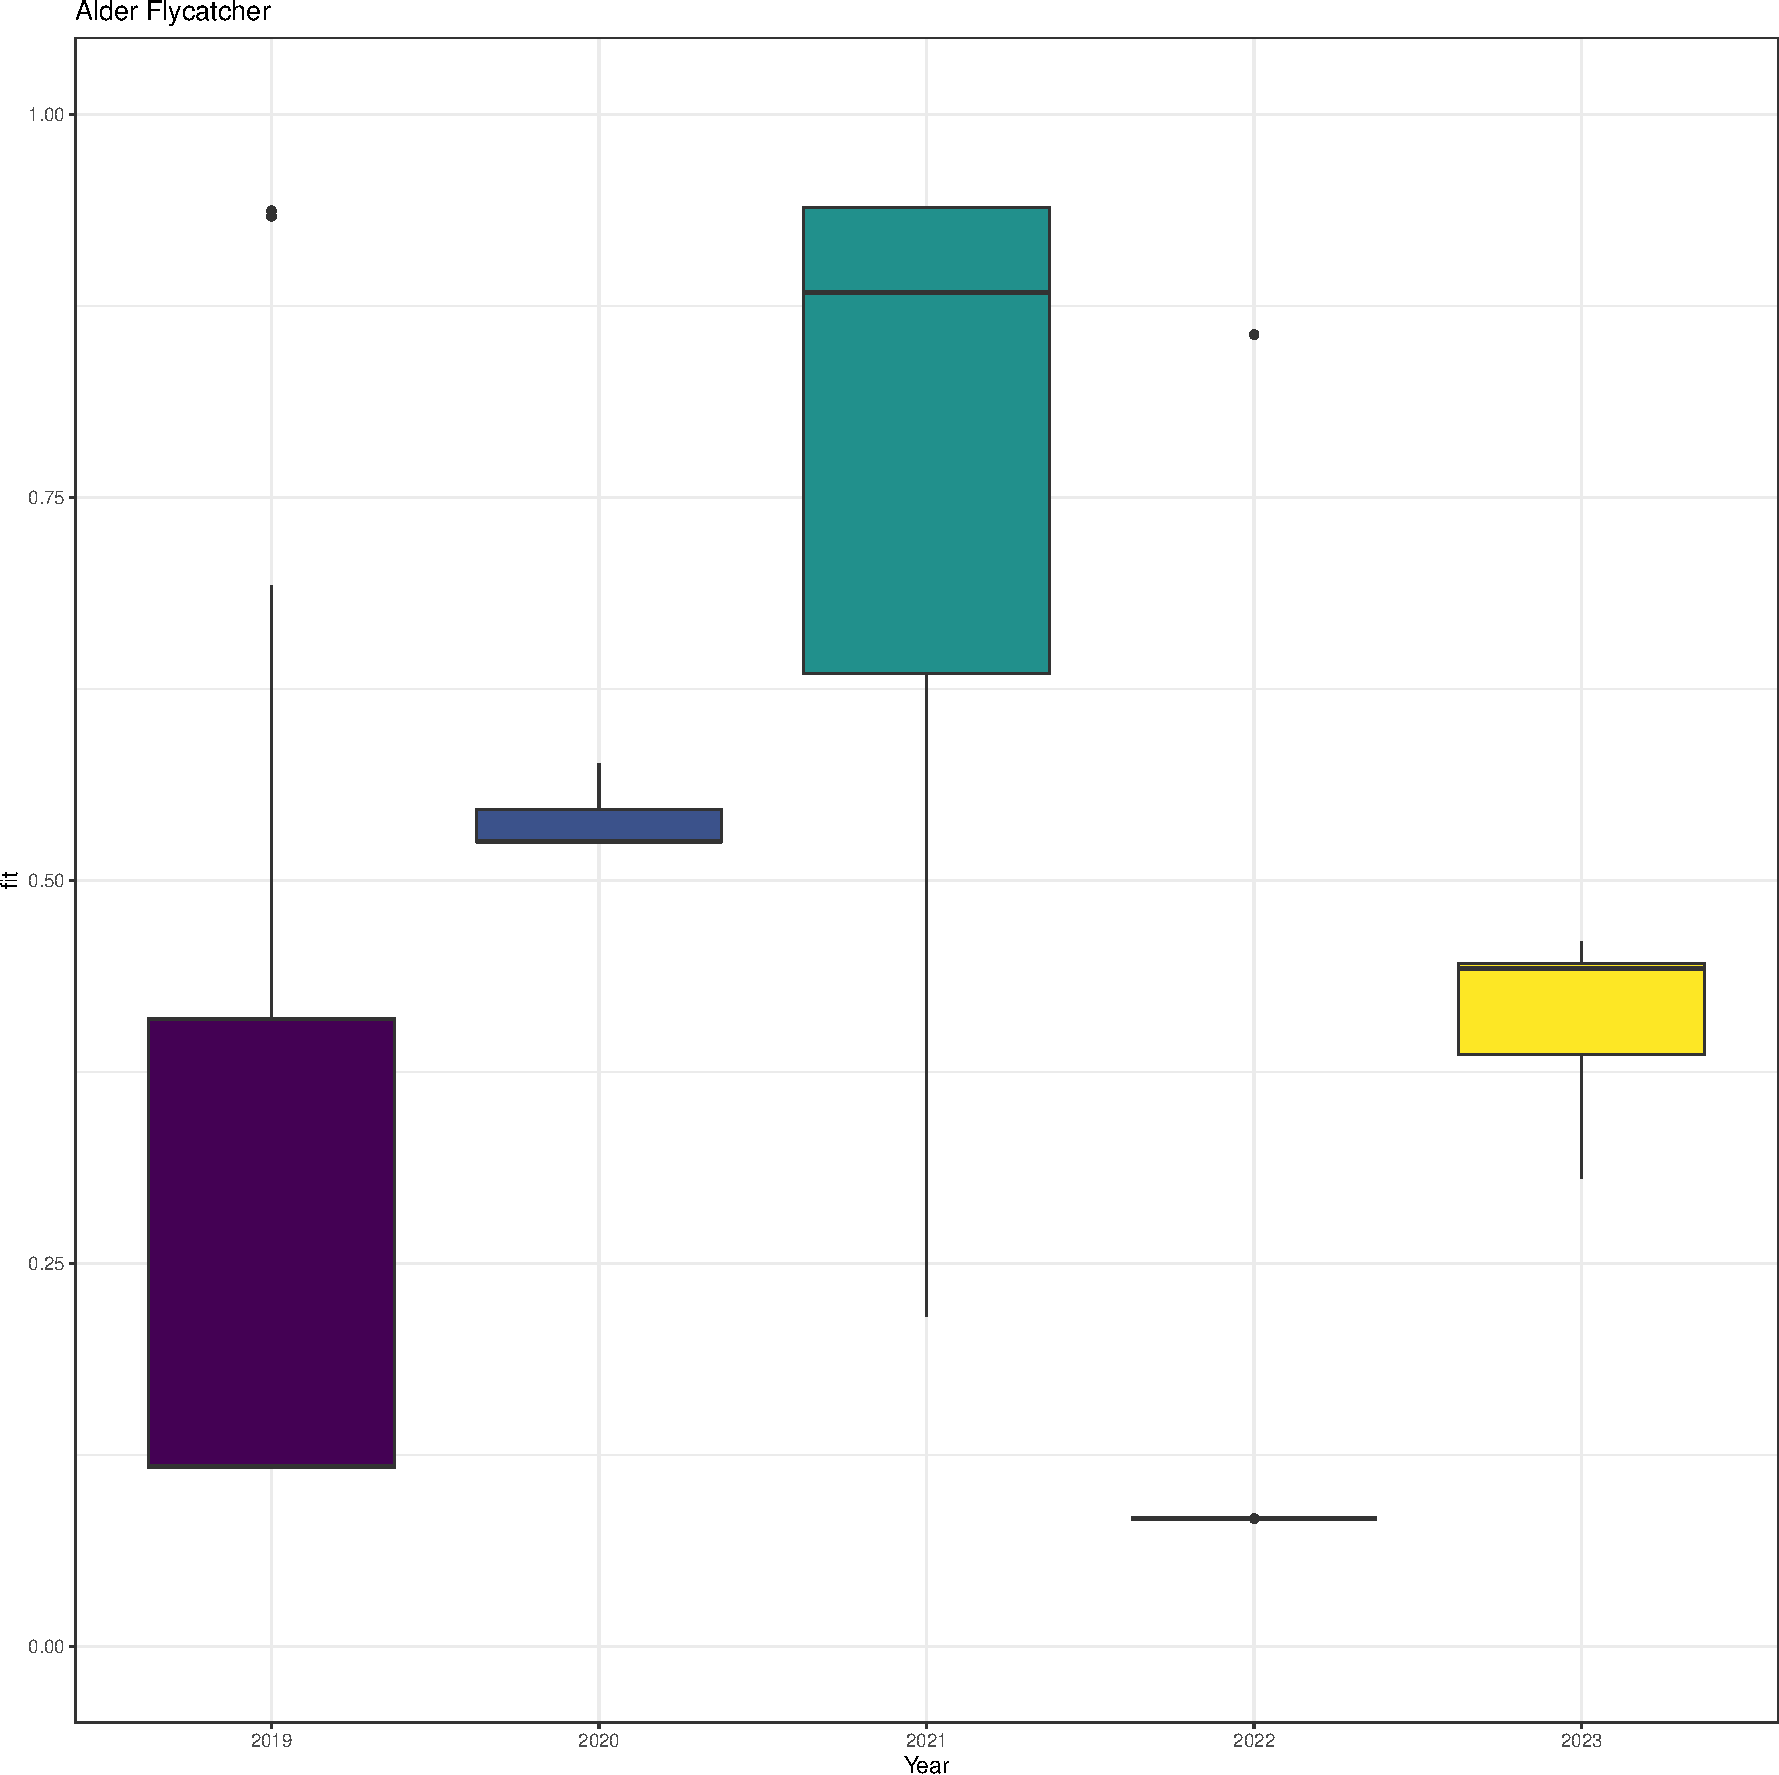
\includegraphics{peinp_files/figure-pdf/fig-spp-occ-tss-1.pdf}

}

\caption{\label{fig-spp-occ-tss}Predicted single-season occupancy of
forest species (Habitat nesting = Treed / Shrubby) within Prince Edward
Island National Park. The data represents the average species occupancy
across all surveyed locations for each respective year.}

\end{figure}

\begin{figure}

{\centering 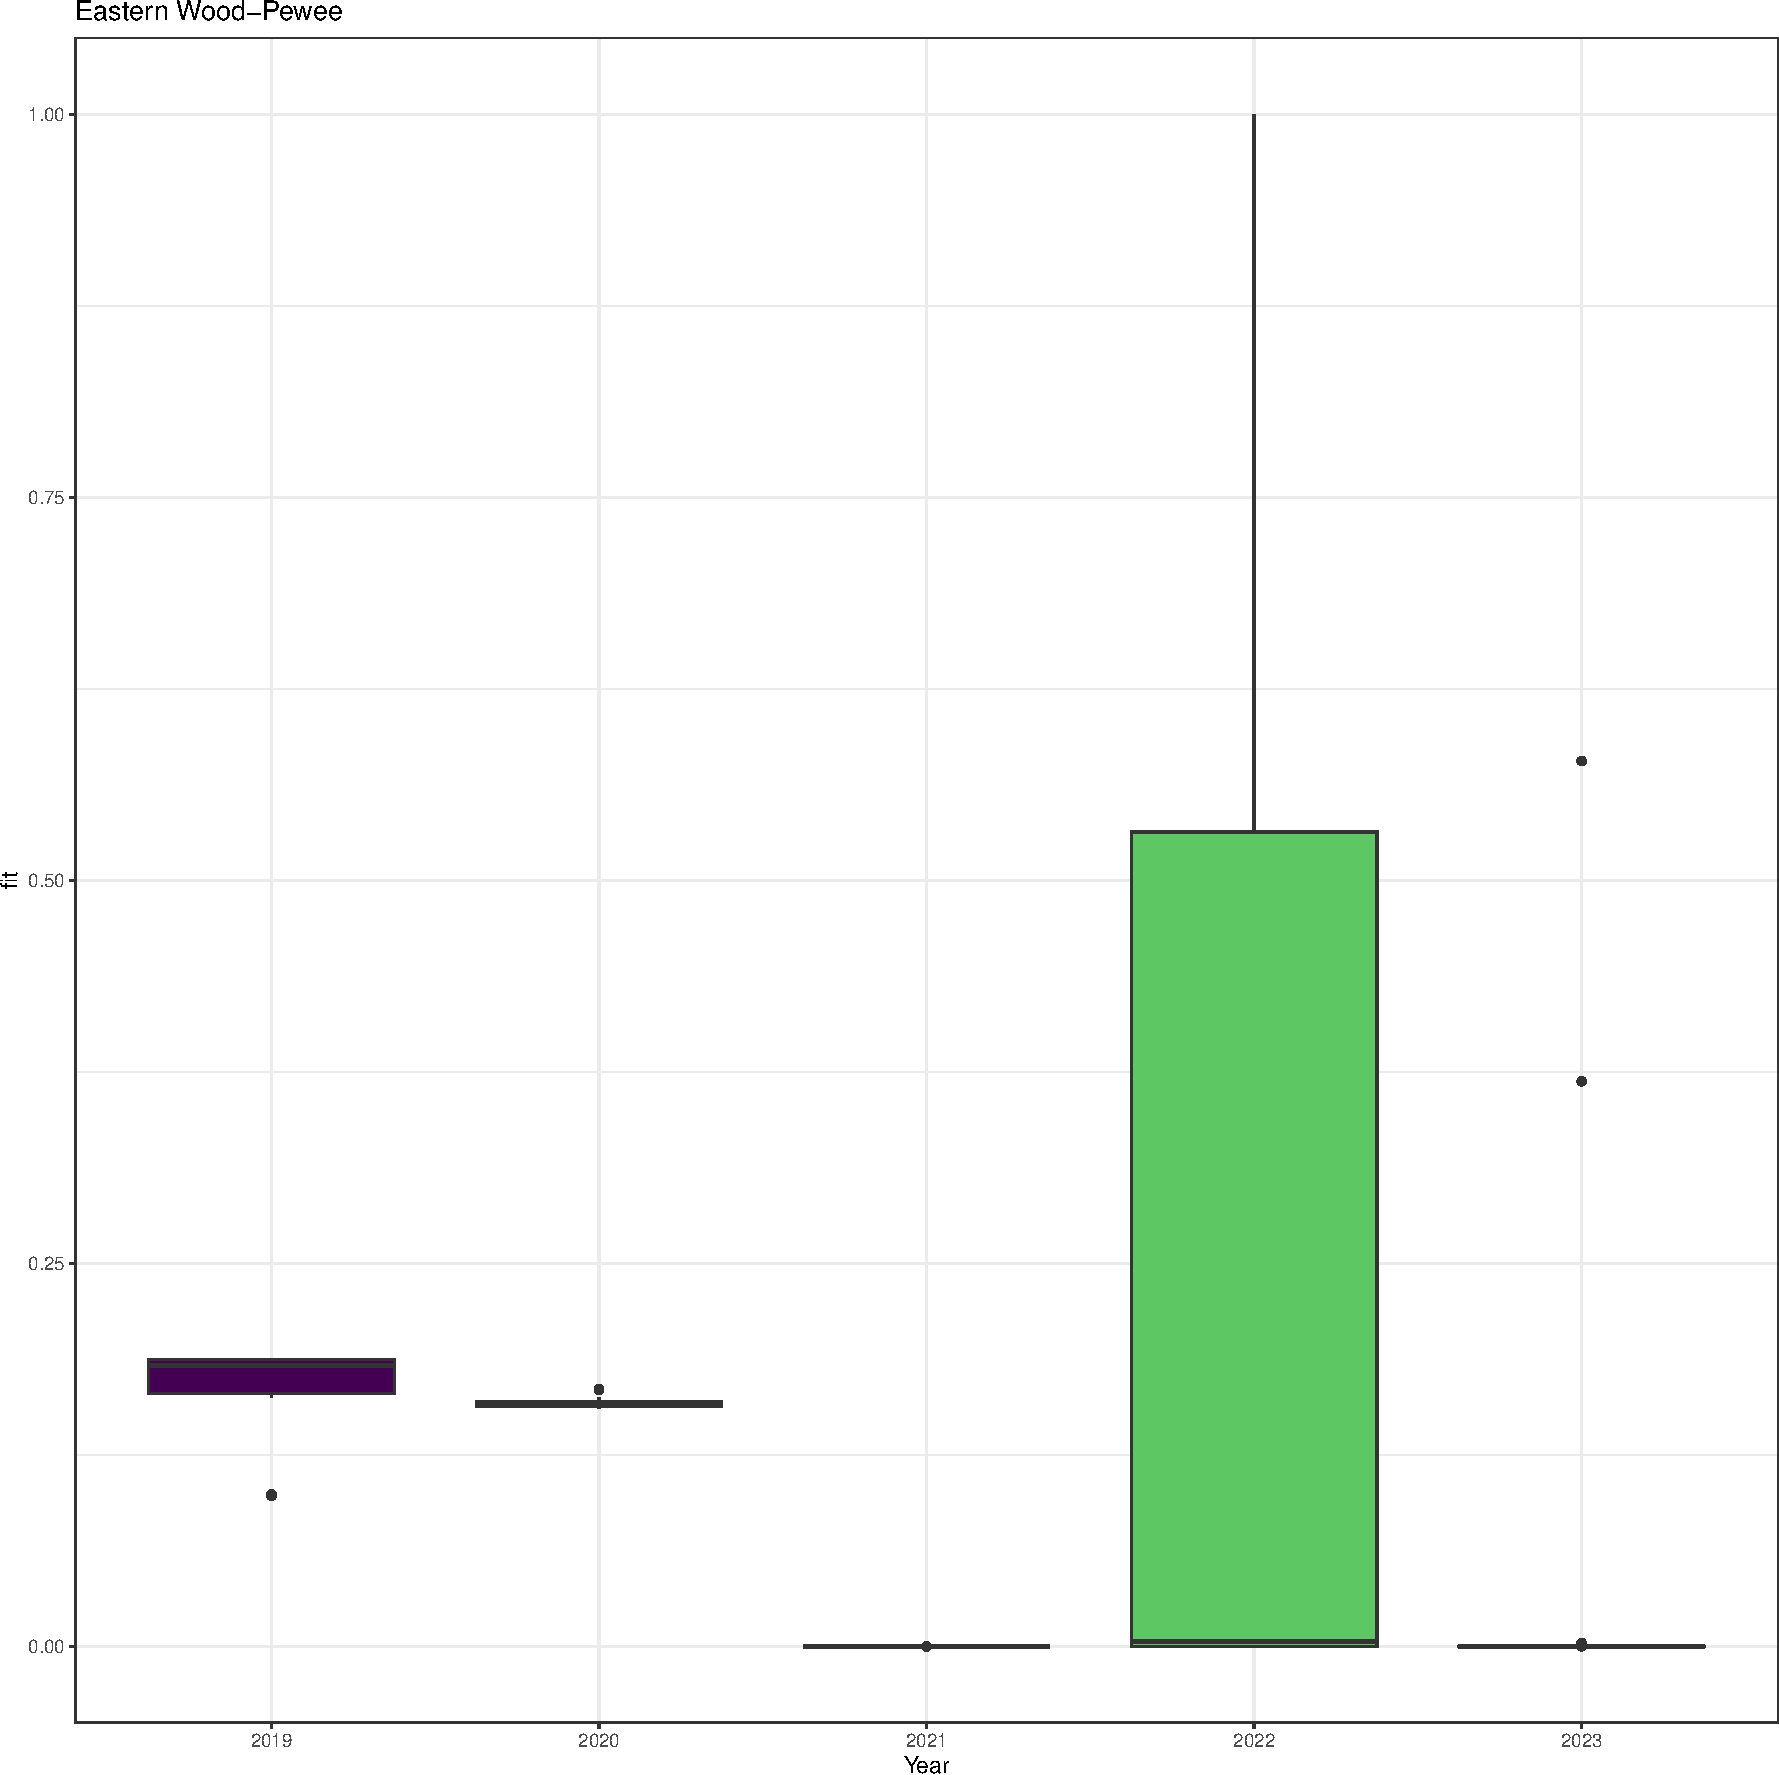
\includegraphics{peinp_files/figure-pdf/fig-spp-occ-open-1.pdf}

}

\caption{\label{fig-spp-occ-open}Predicted single-season occupancy of
forest species (Habitat nesting = Open) within Prince Edward Island
National Park. The data represents the average species occupancy across
all surveyed locations for each respective year.}

\end{figure}

\hypertarget{visual-scanning-1}{%
\subsection{Visual scanning}\label{visual-scanning-1}}

BANS were detected at 3 distinct locations (PENP-BS-1).

\hypertarget{automated-recognition-1}{%
\subsection{Automated recognition}\label{automated-recognition-1}}

We found that there was no advantage to utilizing the recognizer to find
Eastern Wood-Pewee over human transcribing as the species was very
detectable (see \textbf{?@tbl-recog-results}).

\begin{center}\rule{0.5\linewidth}{0.5pt}\end{center}

\hypertarget{amphibians}{%
\subsection{Amphibians}\label{amphibians}}

A total of 7 were detected: SPPE, AMTO, NLFR, GRFG, WOFR, MIFR, BULL. A
preliminary pattern of amphibian activity can be seen in
Figure~\ref{fig-spp-amphs-day} for Green Frog and Spring Peeper where
there were enough detections to generate activity patterns. Spring
peeper activity commenced much earlier than Green Frog although seasonal
patterns are consistent with the species' phenology Lovett
(2013)\marginpar{\begin{footnotesize}\leavevmode\vadjust pre{\protect\hypertarget{ref-lovett2013peepers}{}}%
Lovett, Gary M. 2013. {``When Do Peepers Peep? Climate and the Date of
First Calling in the Spring Peeper (Pseudacris Crucifer) in Southeastern
New York State.''} \emph{Northeastern Naturalist} 20 (2): 333--40.\vspace{2mm}\par\end{footnotesize}},
Ackleh et al.
(2010)\marginpar{\begin{footnotesize}\leavevmode\vadjust pre{\protect\hypertarget{ref-ackleh2010measuring}{}}%
Ackleh, Azmy S, Jacoby Carter, Lauren Cole, Tom Nguyen, Jay Monte, and
Claire Pettit. 2010. {``Measuring and Modeling the Seasonal Changes of
an Urban Green Treefrog (Hyla Cinerea) Population.''} \emph{Ecological
Modelling} 221 (2): 281--89.\vspace{2mm}\par\end{footnotesize}}.

\begin{figure}

{\centering 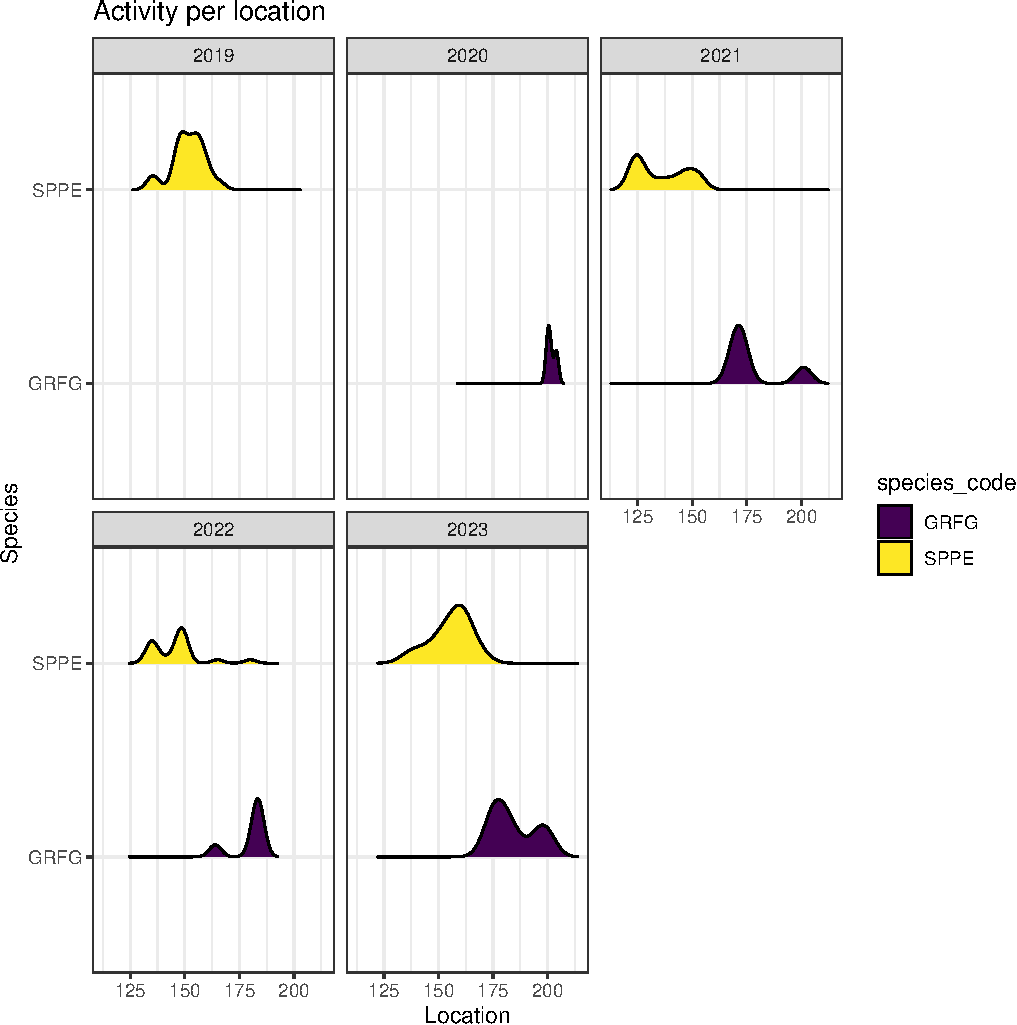
\includegraphics{peinp_files/figure-pdf/fig-spp-amphs-day-1.pdf}

}

\caption{\label{fig-spp-amphs-day}Seasonal and yearly activity plots for
Green Frog and Spring Peeper}

\end{figure}

\begin{center}\rule{0.5\linewidth}{0.5pt}\end{center}

\hypertarget{discussion}{%
\section{Discussion}\label{discussion}}

Considering the natural disturbance effects seen in the Park, species
richness and diversity stayed relatively stable. Individuals of conifer
dominant stands likely moved to more suitable habitat outside the park,
suggesting the potential utility of metapopulation analysis through
passive acoustic monitoring via citizen science. Further analysis may
utilize dynamic occupancy models, multi-species multi-season occupancy
models, or community shifts to describe richness and diversity while
accounting for decreases in species that may rely on specific habitat
structures within the park. Additional geospatial assets could improve
the accuracy of modelling apporaches as well. This study underscores the
efficacy of autonomous recording units (ARUs) as a powerful tool for
monitoring climatic and habitat shifts with a relatively low sample size
and area coverage.

Avian species within the Park forest demonstrate a non-uniform
distribution. Recommendations for optimizing the efficiency and
reliability of the ARU program include:

\begin{itemize}
\tightlist
\item
  Prioritizing monitoring of historical locations, particularly
  emphasizing repeats at PENP-1-1, PENP-1-2, PENP-2-3, PENP-3-1,
  PENP-3-2, PENP-4-1, PENP-4-2, PENP-4-3, PENP-4-4 as baselines for
  evaluating ecological changes over time.
\item
  Adjusting monitoring times to dawn and dusk and extending deployment
  periods to 4-7 days between May 15 and July 15 to maximize
  vocalizations during peak activity periods.
\item
  Regular servicing of ARUs, focusing on testing microphone sensitivity
  degradation to ensure optimal functionality, data reliability, and
  longevity.
\item
  Continuing high-quality verification of tags to create annotated
  datasets for building and automating classifiers within WildTrax.
\end{itemize}




\end{document}
